\documentclass[ALICE,manyauthors]{ALICE_analysis_notes}
%\documentclass[ALICE,manyauthors]{ALICE_scientific_notes}
%
%\newcommand{\jpsi}{\rm J/$\psi$}
%\newcommand{\psip}{$\psi^\prime$}
%\newcommand{\jpsiDY}{\rm J/$\psi$\,/\,DY}
%\newcommand{\dd}{\mathrm{d}}
%\newcommand{\chic}{$\chi_{\rm c}$}
%\newcommand{\ezdc}{$E_{\rm ZDC}$}
%\newcommand{\red}{\textcolor{red}}
%\newcommand{\blue}{\textcolor{blue}}

\usepackage[clockwise]{rotating}
\usepackage{bm}	%for bold math symbols
\usepackage{amssymb}
\usepackage{mathtools}
\usepackage{hyperref}
\usepackage[stable]{footmisc}	% suppress footnotes in table of contents
\usepackage{booktabs}	% nicer tables
\usepackage{caption}
\usepackage{subcaption}	% for subfigures


\newcommand{\slfrac}[2]{\left.#1\right/#2}
\newcommand{\Tr}{\mathrm{Tr}}
\newcommand{\Lag}{\mathcal{L}}
\newcommand{\fsl}[1]{\ensuremath{\mathrlap{\!\not{\phantom{#1}}}#1}}
\newcommand{\lbr}{\lbrace}
\newcommand{\rbr}{\rbrace}
\newcommand{\Ima}{\mathrm{Im}}
\newcommand{\numberthis}{\addtocounter{equation}{1}\tag{\theequation}}	% number equation in unnumbered align/equation environment

%
\begin{document}%
%%%%%%%%%%%%% ptdr definitions %%%%%%%%%%%%%%%%%%%%%
%
%%%%%%%%%%%%%%%  Title page %%%%%%%%%%%%%%%%%%%%%%%%
%
\begin{titlepage}
%
\PHnumber{ALICE-ANA-2014-xxx} 
\PHdate{\today}
%
%%% Put your own title + short title here:
\title{Analysis of light vector mesons in p--p collisions at $\sqrt{s}=$ 13 TeV}
\ShortTitle{Analysis of Light Vector Mesons}   % appears on right page headers
%
\author{Jonathan Kley$^{1}$}
\author{
1. Technical University of Munich\\
}
\author{Email: jonathan.kley@cern.ch}
%
\ShortAuthor{ALICE Analysis Note 2012}      % appears on left page headers, do not change
%
\begin{abstract}
Here goes your abstract
\end{abstract}
\end{titlepage}
\tableofcontents
\newpage

\section{Introduction\footnote{The introduction is mostly based on \cite{ChiSym} with other references used where cited.}}
\label{sec:Introduction}
With the exploration of the phase diagram of nuclear matter has come the idea of the Quark gluon plasma (QGP), a state of matter where confinement is abolished and quarks and gluons can move quasi-freely. However, they still interact strongly, so the medium behaves more like a perfect liquid than a gas. The QGP is created when a critical temperature of $T_c = (154 \pm 9)$ MeV is exceeded \cite{tcrit}. In the laboratory heavy ion collisions are used to deposit a lot of energy in a small spatial volume making it possible to exceed the critical temperature and creating a QGP. After thorough theoretical investigations, experiments in the late 80s started looking for the QGP, but definite traces where only found in the early 2000s by the RHIC experiments at Brookhaven National Laboratory \cite{QGPrhic}. Since then other experiments also joined in on the search for the QGP. After the SPS experiments at CERN could not find any traces of the formation of a QGP, CERN built a dedicated LHC experiment to investigate heavy ion collisions and the QGP, the ALICE experiment \cite{ALICEproposal} which was also used to obtain the data which is analysed here. \\
Because of the short life time (of $O(10 \frac{fm}{c})$ \cite{QGPlifetime}) of the QGP and its strongly interacting nature, it is very difficult to gain information about the properties of the QGP. This is mainly because particles either live too long to decay inside the QGP and therefore lose their information. Or if they decay inside the QGP, their decay products might interact strongly and lose the information they carry about the QGP through scattering in the QGP. So, the most important probes to investigate the QGP are short-lived particles which decay into particles which only interact electromagnetically. One candidate are vector mesons which carry the same quantum numbers as photons ($J^P = 1^{-}$) and couple to them (and therefore effectively to dileptons) as explained by the vector-dominance model. The dileptons are a very clean experimental probe and can be identified with high precision in the ALICE TPC. \\
One of the most interesting aspects of the QGP is the possible restoration of the chiral symmetry which might also be connected to a phase transition in the phase diagram of nuclear matter. There are many implications of this possible restoration of chiral symmetry on the particle spectrum of QCD which in reverse can also be used to check if our fundamental theory of the strong interaction - QCD - is correct. One system which should in theory be affected by the restoration of chiral symmetry and also  is the $\rho$-$a_1$ system. If chiral symmetry is present these two particles are related to each other which has consequences on their so-called spectral functions. \\
This work is a feasibility study of the measurement of the $a_1$ meson at the ALICE experiment in pp collisions. Along the $a_1$ meson we also try to identify vector mesons which appear in the same decay channels to double check our results. \\
This paper is structured as follows. In section \ref{sec:Introduction} I will discuss the chiral symmetry of QCD and its consequences in more detail, also including implications on the $\rho$-$a_1$ system. I will then discuss the details of the data analysis in section \ref{sec:Analysis} including the analysis strategy and particle cuts and event selection. Finally in section \ref{sec:Results}, I will discuss the results and give a quick outlook in section \ref{sec:Outlook}.

\subsection{The QCD Lagrangian}
To understand the effects of the strong interaction we use the theory which has been proven most successful in this matter in the end of the last century: QCD. We start from the classic Lagrangian of QCD with 3 flavours which is the unique Lagrangian which is invariant under a gauged SU(3) symmetry
\begin{equation}
\label{eqn:LQCD}
\Lag_{QCD} = \bar{\psi}_i \left( i\gamma_{\mu} D^{\mu} - m \right)_{ij} \psi_j - \frac{1}{4} G_{\mu\nu}^a G^{\mu\nu}_a
\end{equation}
where $\psi = \left( u,d,s \right)$ are the quark fields, $D^{\mu} = \partial^{\mu} -igA^{\mu}$ is the covariant derivative in the fundamental representation and $G_{\mu\nu}^a = \partial_{\mu}A_{\nu} - \partial_{\nu}A_{\mu} + g f^{abc} A_{\mu}^b A_{\nu}^c$ is the field strength of the gluon fields $A_{\mu}^a$ with the structure constants $f^{abc}$ of SU(3). \\
Following the usual procedure of perturbative renormalization we can calculate the $\beta$-function in QCD. At 1-loop order it is given by \cite{QCDEllis}
\begin{equation}
\label{eqn:beta}
\beta(\alpha_S) = \mu_R^2 \frac{d\alpha_S}{d\mu_R^2} = - \left( 11 - \frac{2}{3} n_f \right) \frac{\alpha_S^2}{4\pi} + O(\alpha_S^3)  \equiv - \beta_0 \frac{\alpha_S^2}{4\pi} + O(\alpha_S^3)
\end{equation}
where $n_f$ is the number of flavours and $\beta_0$ the 1-loop $\beta$-function coefficient.
Solving the differential equation in eqn. \ref{eqn:beta} in terms of the renormalized scale $\mu_R^2$ we get an expression for the running coupling in QCD. Using the 1-loop expression we get
\begin{equation}
\label{eqn:alpha}
\alpha_S(\mu) = \frac{4\pi}{\beta_0 \log\frac{\mu^2}{\Lambda^2}} 
\end{equation}
where $\Lambda$ is the QCD scale and we fixed $\alpha(\mu) \overset{\mu \rightarrow \Lambda}{\longrightarrow} \infty$. A plot of the running coupling along with the most recent measurements can be seen in fig. \ref{fig:alpha}. \\
From eqn. \ref{eqn:alpha} it is obvious that perturbation theory is not applicable at energy scales close to the fundamental scale of our theory. Unfortunately this is the regime we are interested in, so we have to think of another way to approach scales $\mu < \Lambda_{QCD}$. 
\begin{figure}[t]
	\centering
	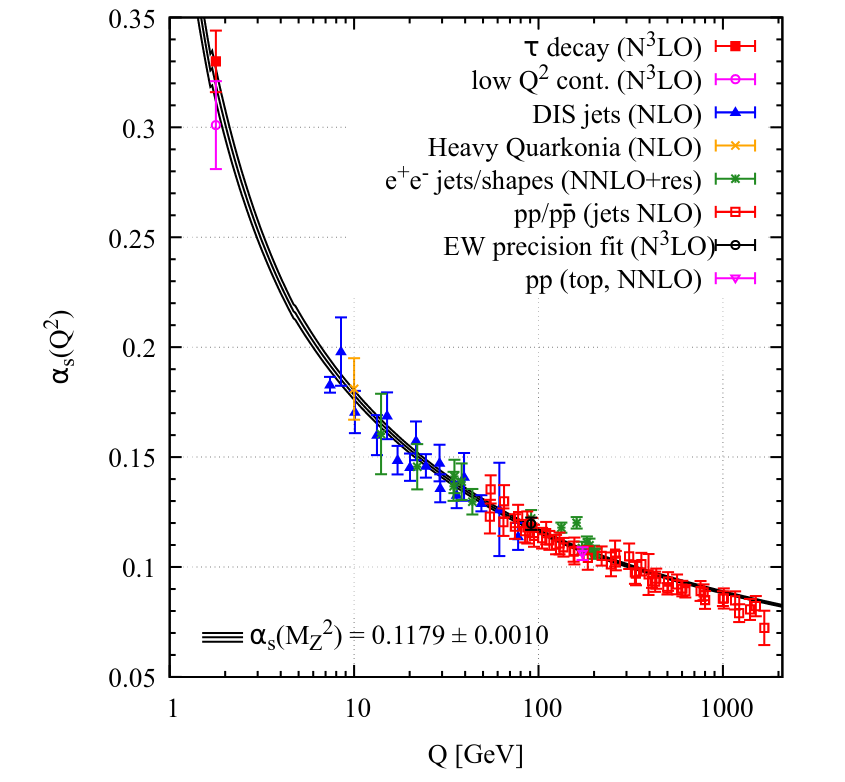
\includegraphics[width=0.55\textwidth]{Figures/alphaQCD}
	\caption{The running coupling of QCD \cite{PDG2018}. Summary of measurements of $\alpha_S$ as a function of the scale $Q$. The order in QCD perturbation theory which was used in the calculation is indicated in brackets.}
	\label{fig:alpha}
\end{figure}
\subsection{Chiral Symmetry of QCD}
One of the ways to approach regimes where $\mu < \Lambda_{QCD}$ is to build an effective Lagrangian based on the symmetries of the fundamental Lagrangian of QCD. In this section we investigate this approach and see which implications it has for the particle spectrum of the theory. \\
We start from the Lagrangian of QCD in eqn. \ref{eqn:LQCD}. Of particular interest to us for the chiral symmetry is the quark term in the Lagrangian which can be split into two parts
\begin{equation}
\Lag_{\mathrm{quarks}} = \bar{\psi} i\gamma_{\mu} D^{\mu} \psi - m \bar{\psi} \psi \equiv \Lag + \delta\Lag
\end{equation}
The suggestive names will make sense in a second. 
Since the doublet of quark fields in $\Lag$ are contracted in an inner product the Lagrangian is invariant under an inner symmetry. In our case this is a U(2) symmetry for both chiralities, so U(2)$_L \times$ U(2)$_R$ in total. We can also think of the symmetries in terms of axial and vector currents instead of left and right handed currents which is more useful in this analysis, so the symmetry group is U(2)$_V \times$ U(2)$_A$. We only consider the SU(2) part of both subgroups, since U(1)$_V$ can be identified with baryon number conservation and U(1)$_A$ is anomalous because th, so it is not a real symmetry of our theory. Let us consider the following SU(2) transformations
\begin{align}
& U_V = \exp \left(-i \alpha^i \frac{\sigma^i}{2} \right) \approx 1 - i\alpha^i \frac{\sigma^i}{2} \in SU(2)_V & \label{eqn:Vtrafo} \\
& U_A = \exp \left(-i \gamma_5 \alpha^i \frac{\sigma^i}{2} \right) \approx 1 - i \gamma_5 \alpha^i \frac{\sigma^i}{2} \in SU(2)_A & \label{eqn:Atrafo}
\end{align}
of the quark fields and their action on $\Lag$
\begin{equation}
\Lag = i \psi^{\dagger} \gamma_0 \gamma^{\mu} D_{\mu} \psi \overset{U_V}{\longrightarrow} i \left( U_V \psi \right)^{\dagger} \gamma_0 \gamma^{\mu} D_{\mu} U_V \psi = i \psi^{\dagger} e^{+i \alpha^i \frac{\sigma^i}{2}} \gamma_0 \gamma^{\mu} D_{\mu} e^{-i \alpha^i \frac{\sigma^i}{2}} \psi = i \bar{\psi} \fsl{D} \psi
\end{equation}
and
\begin{equation}
\Lag = i \psi^{\dagger} \gamma_0 \gamma^{\mu} D_{\mu} \psi \overset{U_A}{\longrightarrow} i \left( U_A \psi \right)^{\dagger} \gamma_0 \gamma^{\mu} D_{\mu} U_A \psi = i \psi^{\dagger} e^{+i \alpha^i \gamma_5 \frac{\sigma^i}{2}} \gamma_0 \gamma^{\mu} D_{\mu} e^{-i \gamma_5 \alpha^i \frac{\sigma^i}{2}} \psi = i \bar{\psi} \fsl{D} \psi
\end{equation}
where we used $\lbr \gamma^{\mu},\gamma_5 \rbr = 0 = \left[ D^{\mu},\gamma_5 \right]$ and $\gamma_5^{\dagger} = \gamma_5$.
So $\Lag$ is invariant under both $U_V$ and $U_A$.
The corresponding currents are
\begin{align}
& j_{\mu}^i = \bar{\psi} \gamma_{\mu} \frac{\sigma^i}{2} \psi & \label{eqn:jV} \\
& j_{5\mu}^i = \bar{\psi} \gamma_{\mu} \gamma_5 \frac{\sigma^i}{2} \label{eqn:jA} \psi & 
\end{align}
Now we can check the effect of the transformations on $\delta \Lag$
\begin{equation}
\delta \Lag = - m \psi^{\dagger}\gamma^0 \psi \overset{U_V}{\longrightarrow} - m \left( U_V \psi \right)^{\dagger}\gamma^0 U_V \psi = - m \psi^{\dagger} e^{+i\alpha^i \frac{\sigma^i}{2}} \gamma^0 e^{-i\alpha^i \frac{\sigma^i}{2}} \psi = - m \bar{\psi} \psi
\end{equation}
and 
\begin{equation}
\delta \Lag = - m \psi^{\dagger}\gamma^0 \psi \overset{U_A}{\longrightarrow} - m \left( U_A \psi \right)^{\dagger}\gamma^0 U_A \psi = - m \psi^{\dagger} e^{+i \gamma_5 \alpha^i  \frac{\sigma^i}{2}} \gamma^0 e^{-i \gamma_5 \alpha^i \frac{\sigma^i}{2}} \psi = - m e^{2i \gamma_5 \alpha^i \frac{\sigma^i}{2}} \bar{\psi} \psi \neq \delta \Lag
\end{equation}
where we used the same identities as above. We see that the mass term is not invariant under axial transformations while it is left invariant by vector transformations. The axial symmetry is therefore explicitly broken by the quark mass term. But as long as the quark masses are smaller than the scale of our theory we can still use the symmetry as an approximate symmetry. This is indeed the case, since $m_u,m_d \sim O(5 \ \mathrm{MeV}) \ll \Lambda_{QCD} \simeq 200 \ \mathrm{MeV}$.

\subsection{Spontaneous Chiral Symmetry Breaking}
With our 2 quark fields we can now build bosonic fields that have the quantum numbers of the mesons in nature. We find
\begin{align*}
& \mathrm{pion-like \ state:} \ \vec{\pi} \equiv i \bar{\psi} \vec{\sigma}\gamma_5 \psi; \qquad \mathrm{sigma-like \ state:} \ \sigma \equiv \bar{\psi}\psi & \\
&\mathrm{rho-like \ state:} \ \vec{\rho}_{\mu} \equiv \bar{\psi} \vec{\sigma}\gamma_{\mu} \psi; \qquad a_1\mathrm{-like \ state:} \ \vec{a}_{1 \mu} \equiv \bar{\psi} \vec{\sigma}\gamma_{\mu}\gamma_5 \psi &
\end{align*}
Of particular interest to us will be the $\rho$ and the $a_1$ states because they correspond to the conserved currents from eqn. \ref{eqn:jV} and \ref{eqn:jA} and therefore seem to be closely related to the chiral symmetry. Let us see now how these particles transform under the chiral transformations in infinitesimal form, so we can understand the symmetry better.
Starting with the $\pi$ state and with the vector transformation from eqn. \ref{eqn:Vtrafo} we get
\begin{align*}
i \bar{\psi} \sigma^i \gamma_5 \psi & \overset{U_V}{\longrightarrow} i \left( U_V \psi \right)^{\dagger} \gamma^0 \sigma^i\gamma_5 U_V \psi = i \bar{\psi} \sigma^i\gamma_5 \psi + \alpha^j \left( \bar{\psi} \sigma^i \frac{\sigma^j}{2} \gamma_5 \psi - \bar{\psi} \frac{\sigma^j}{2} \sigma^i \gamma_5 \psi \right) + O(\alpha^2) = & \\
& = i \bar{\psi} \sigma^i\gamma_5 \psi + i \alpha^j \epsilon^{ijk} \bar{\psi} \sigma^k\gamma_5 \psi & \numberthis
\end{align*}
where we have used the $SU(2)$ algebra $\left[\sigma^i,\sigma^j \right] = 2i \epsilon^{ijk} \sigma^k$. We can do similar calculations for all of the other states as well and get for the vector transformations
\begin{align}
\vec{\pi} \overset{U_V}{\longrightarrow} & \vec{\pi} + \vec{\alpha} \times \vec{\pi} & \\
\sigma \overset{U_V}{\longrightarrow} & \sigma & \\
\vec{\rho}_{\mu} \overset{U_V}{\longrightarrow} & \vec{\rho}_{\mu} + \vec{\alpha} \times \vec{\rho}_{\mu} & \\
\vec{a}_{1 \mu} \overset{U_V}{\longrightarrow} & \vec{a}_{1 \mu} + \vec{\alpha} \times \vec{a}_{1 \mu}
\end{align}
Which is also what we expect when we identify $SU(2)_V$ with isospin. $\vec{\pi}$, $\vec{\rho}_{\mu}$ and $\vec{a}_{1 \mu}$ are all in the fundamental representation of isospin and are therefore changed by an isospin rotation. Whereas, $\sigma$ is a scalar under isospin and is therefore not affected. \\
However, under the axial transformations the particles mix as follows
\begin{align}
\vec{\pi} \overset{U_A}{\longrightarrow} & \vec{\pi} + \vec{\alpha} \sigma & \\
\sigma \overset{U_A}{\longrightarrow} & \sigma - \vec{\alpha} \cdot \vec{\pi} & \\
\vec{\rho}_{\mu} \overset{U_A}{\longrightarrow} & \vec{\rho}_{\mu} + \vec{\alpha} \times \vec{a}_{1 \mu} & \\
\vec{a}_{1 \mu} \overset{U_A}{\longrightarrow} & \vec{a}_{1 \mu} - \vec{\alpha} \times \vec{\rho}_{\mu}
\end{align}
Since 2 pairs of particles are rotated into each other by axial rotations, this suggests that these particles have the \textit{same} mass or after the explicit breaking of $SU(2)_A$ by the quark mass term at least a \textit{similar} mass. But this does not seem to be the case in nature, since e.g. the $a_1$ has a mass of $m_{a_1} \simeq 1260$ MeV which is almost double the mass of the $\rho$ meson with a mass of $m_{\rho} \simeq 770$ MeV. \\
So, clearly $m_{a_1} \not\simeq m_{\rho}$ and $SU(2)_A$ can not be a symmetry of the vacuum and must therefore be spontaneously broken: $SU(2)_V \times SU(2)_A \rightarrow SU(2)_V$. This can also be seen from the vacuum expectation value (VEV) of the term $\bar{\psi}\psi$ 
\begin{equation}
\label{eqn:vev} 
\langle 0 | \bar{\psi} \psi | 0 \rangle \overset{U_A}{\longrightarrow} \langle 0 |   \bar{\psi} e^{-2i \gamma_5 \alpha^i \frac{\sigma^i}{2}} \psi | 0 \rangle
\end{equation}
which would be invariant if the vacuum was invariant: $U_A | 0 \rangle = e^{-i \gamma_5 \alpha^i \frac{\sigma^i}{2}} | 0 \rangle = | 0 \rangle$. However, this is not the case in nature as we just discussed. Therefore, $SU(2)_A$ must be spontaneously broken and $\bar{\psi}\psi$ - the so-called chiral condensate - must develop a vacuum expectation value $\langle \bar{\psi}\psi \rangle = - \left( 250 \text{MeV} \right)^3$. We can use the VEV as an order parameter for the breaking of $SU(2)_A$. If the symmetry is not broken the VEV is zero and if we have a finite VEV the symmetry is broken as we expect from an order parameter. \\
We can now interpret the three spin-0 particles $\vec{\pi}$ from above as the Goldstone bosons of the spontaneously broken $SU(2)_A$. If $U(1)_A$ wasn't anomalous, we could identify the $\sigma$ as its Goldstone boson, which in the case of three flavours can be identified with the $\eta'$. \\
We could now turn on the usual machinery for spontaneously broken symmetries and construct the effective Lagrangian of the pions. But since we don't do any original calculations in this paper, let us skip that and look at some implications of the spontaneous symmetry breaking and the possible return of the symmetry. Especially in the for the vector mesons whose field configurations correspond to the conserved currents.

\subsection{Effects of Hot and Dense Matter on Chiral Symmetry}
In this section I want to discuss the possible effects of hot and dense matter - like a QGP - on observables. In our case only the temperature dependence is interesting, since the ALICE experiment operates at zero baryon chemical potential. The QGP in ALICE is created by depositing as much energy as possible in a small spatial volume and then hoping to reach a temperature $T > T_c$. \\
Let us start with the discussion of the order parameter of chiral symmetry which we just defined in eqn. \ref{eqn:vev}. Gerber and Leutwyler showed that up to 3-loop order the temperature dependence of $\langle \bar{\psi} \psi \rangle$ for $T < T_c$ and massless quarks is given by \cite{OrdPar3loop}
\begin{equation}
\frac{\langle \bar{\psi} \psi \rangle(T)}{\langle \bar{\psi} \psi \rangle(T=0)} = 1 - x - \frac{1}{6} x^2 - \frac{16}{9} x^3 \ln \frac{T}{\Lambda_q}
\end{equation}
where $x = \frac{T^2}{8f^2}$, the relevant temperature scale is $\sqrt{8}f \simeq 250$ MeV with $f$ the pion decay constant in the chiral limit and $\Lambda_q = (470 \pm 110)$ MeV. We can see a clear trend of a decreasing order parameter for increasing temperature which suggests a restoration of chiral symmetry if the trend continues. \\
The temperature dependence over a bigger interval can be obtained from lattice QCD. The results of one such calculation can be found in fig. \ref{fig:ordparlat}. Here we can see that the trend indeed continues and chiral symmetry seems to be restored in a QGP.
\begin{figure}[b]
	\centering
	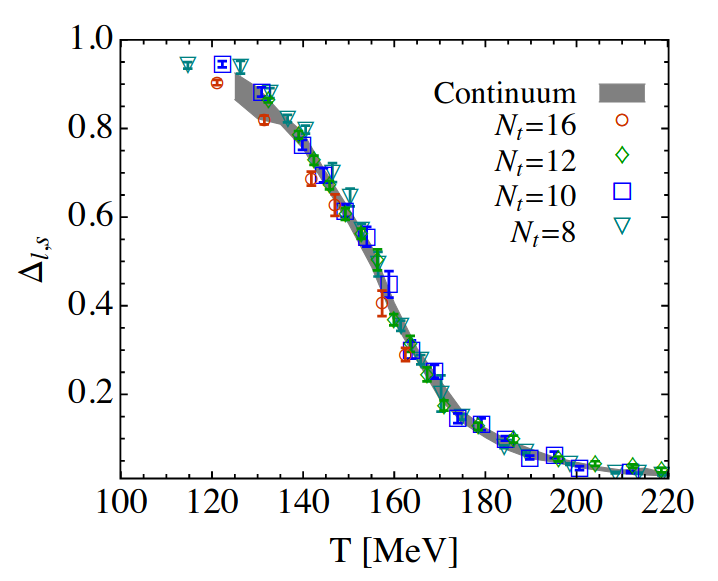
\includegraphics[width=0.45\textwidth]{Figures/ChiralOrderParameterLattice}
	\caption{Lattice calculation of subtracted chiral condensate which is defined as $ \Delta_{l,s} = \frac{\langle \bar{\psi} \psi \rangle_{l,T} - \frac{m_l}{m_s} \langle \bar{\psi} \psi \rangle_{s,T}}{\langle \bar{\psi} \psi \rangle_{l,0} - \frac{m_l}{m_s} \langle \bar{\psi} \psi \rangle_{s,0}}$ with $l = u,d$ \cite{OrdParLat}.}
	\label{fig:ordparlat}
\end{figure}
This of course has consequences on the things we discussed earlier. Let us have a look another look at the axial and vector currents from eqn. \ref{eqn:jV} and \ref{eqn:jA} transforming under the axial transformation
\begin{equation}
\vec{j}^V_{\mu} = \psi^{\dagger} \gamma^0 \gamma_{\mu} \frac{\vec{\sigma}}{2} \psi \overset{U_A}{\longrightarrow} U_A^{\dagger} \bar{\psi} \gamma_{\mu} \frac{\vec{\sigma}}{2} U_A \psi = U_A^{\dagger} \vec{j}^V_{\mu} U_A
\end{equation}
With this transformation rule we can calculate transformation of the correlator
\begin{equation}
\Pi_{\mu\nu} (q) = i \int d^4x e^{iq \cdot x} \langle 0 | \mathcal{T} j^V_{\mu}(x)j^V_{\nu}(0) | 0 \rangle
\end{equation}
in which we can see the vector mesons as resonances. Then assuming chiral symmetry is restored - so $U_A | 0 \rangle = | 0 \rangle$ - we get for the transformation of the correlator
\begin{equation}
\Pi_{\mu\nu}(q) \overset{U_A}{\longrightarrow} i \int d^4x e^{iq \cdot x} \langle 0 | \mathcal{T} U_A^{\dagger} j^V_{\mu}(x) U_A U_A^{\dagger} j^V_{\nu}(0) U_A | 0 \rangle \overset{U_A | 0 \rangle = | 0 \rangle}{=} i \int d^4x e^{iq \cdot x} \langle 0 | \mathcal{T} j^V_{\mu}(x)j^V_{\nu}(0) | 0 \rangle = \Pi_{\mu\nu} (q)
\end{equation}

NOT WHAT WE WANT TO CALCULATE!!! WHAT WE WANT jA = UjV and then <jVjV> = <jAjA> weinberg sumrule Rennecke

"Current correlation functions, QCD sum rules and vector mesons in baryonic matter"



We also see that \cite{ChiPart} correlations function change but might be restored in medium and/or high temperatures. Also from axial trafo of mesons which can be identified with currents
\begin{equation}
j_V \overset{U_A}{\longrightarrow} j_V + \alpha j_A
\end{equation}


show density and temperature dependency of chiral condensate 
might vanish in QGP --> chiral restoration

theory of correlation functions: formula 1 in "Chiral symmetry and mixing of axial and vector correlators in matter" (if chiral symmetry restored we can use jV = UA jA?)



rho has been studied a lot (see below) while there are only few results for a1 (mostly from tau decays)

CERES experiment \cite{CERESrho} and NA60 experiment \cite{NA60rho} reported broadening scenario for $\rho$.
\section{Data Analysis}
\label{sec:Analysis}
\subsection{Analysis Strategy}
\begin{table}[b]
\centering{
\begin{tabular}{@{} rcl @{}}
  \toprule
  Particle & Decay Mode & Branching Ratio \\ \midrule
  $a_1$ & \qquad \qquad \qquad \qquad $\pi^{0}\gamma$ \qquad \qquad \qquad \qquad & $(0.15 \pm 0.07)$\% \\ 
  $a_1$ & \qquad \qquad $\pi^0\pi^{+}\pi^{-}$ \qquad \qquad & seen, BR not known\\ \midrule
  $\omega$ & \qquad \qquad $\pi^{0}\gamma$ \qquad \qquad & $(8.40 \pm 0.22)$\% \\
  $\omega$ & \qquad \qquad $\pi^0\pi^{+}\pi^{-}$ \qquad \qquad & $(89.3 \pm 0.06)$\% \\ \midrule
  $\eta$ & \qquad \qquad $\pi^0\pi^{+}\pi^{-}$ \qquad \qquad & $(22.92 \pm 0.28)$\% \\ \midrule
  $\rho$ & \qquad \qquad $\pi^{+}\pi^{-}$ \qquad \qquad & $\sim 100$\% \\
  \bottomrule 
\end{tabular}
}
\caption{Decay modes of the $a_1$ meson and control modes $\omega,\eta$ and $\rho$ \cite{PDG2018}}
\label{tab:pdg}
\end{table}
In the first section, we got a first insight on the importance of the $a_1$-$\rho$ system as a probe for chiral symmetry restoration. Eventually, one would like to measure the $a_1$ in heavy-ion collisions decaying only into electromagnetically interacting particles so effects of the QGP would be visible. Since this is a feasibility study of the measurement of the $a_1$ in the ALICE detector we use the decay modes which can be most easily tracked with the detector. With its TPC the ALICE detector has a very precise tool to trace charged particles. The ALICE detector also offers three calorimeters, the PHOS, the EMCAL and the DCAL which can be used to measure the energy of neutral particles. Looking at table \ref{tab:pdg} what we want to do to analyse the $a_1$ in the $\pi^0 \gamma$ channel, is to hope for the neutral pion to decay into two photons (which happens in approximately 99\% of the cases \cite{PDG2018}) and then measure them along with the other photon from the $a_1$ decay with the calorimeters. The other option is two hope for all of the photons to decay in the detector material and then use the dielectron pairs from the conversion to reconstruct the $a_1$. For the $\pi^0 \pi^{+}\pi^{-}$ decay channel we can use the tracking capabilities of the TPC to trace the charged pions and then do the same procedure as for the other decay channel for the neutral pion. \\
Both techniques obviously have their advantages and disadvantages. The photon conversion method (PCM) works very well at low transverse momenta. This is because it uses the tracks of the charged particles to reconstruct the photon. Obviously the track of a particle with lower momentum will be bent more, i.e. have a smaller radius of curvature, then a particle with high momentum. Therefore a smaller radius of curvature should mean a better, i.e. smaller, resolution. We can estimate a resolution with $\sigma_{PCM} \sim R = \frac{p_T}{qB}$ by setting the centrifugal force of a particle equal to the Lorentz force in a magnetic field and assuming $p \simeq p_T$. For constant magnetic field and charge this estimate of the resolution obviously gets better with lower $p_T$. Another advantage is that particles can be identified relatively easily, e.g. using their specific energy loss in the TPC. One of the biggest disadvantages of PCM is the conversion probability. The conversion probability for ALICE for the integrated detector material for $R<180$ cm and $|\eta|<0.9$ is about 8.5\% \cite{ALICEPerfRep}. If we then have to take this to the power of three for the $\pi^0\gamma$ channel, the already low probability to find the $a_1$ is dampened even more. \\
For the calorimeters we can also make a quick estimation of the resolution. If we assume Gaussian distribution of the response (variance scaling like $\sqrt{N}$ where N is the number of events) the relative resolution scales like $\frac{\sigma}{N} = \frac{\sqrt{N}}{N} = \frac{1}{\sqrt{N}}$. If we also assume that each photon carries some average energy $E \sim p_T$ in the calorimeter we get as an estimate $\sigma_{Calo} \sim \frac{1}{\sqrt{p_T}}$. This obviously gets better with high $p_T$. One disadvantage is that all the particles that make it past the other detectors will end up in the calorimeters which are located at the outermost radii of the whole apparatus. We also have to identify the particles which can be done by using first of all a charged particle veto to get rid of all charged particles and then e.g. using the shower shape of the  decaying particle in the calorimeter. \\
In table \ref{tab:pdg} one can also find a few other particles which have the same decay modes as the $a_1$: the $\omega$ and the $\eta$ and also the $\rho$ which should appear in the charged pion mass spectrum of the other decays. We can use these particle decays to see if our analysis is sensible.

\subsection{Event Selection}
For the event selection we took all of the  13 TeV pp events into account which are flagged by the minimum bias INT7 trigger which requires a coinciding signal in the V0 detector arrays. We also required the detectors we used in the analysis to provide a good signal for the flagged events. Then we performed the basic pile-up rejection to get rid of events where several proton collisions happened in a too short time window for the single events to still be resolved. Finally, we required the z-coordinate of the primary vertex to be within 10 cm of the nominal interaction point and required the primary vertex to have at least one contributor. After this procedure about events where left. \\


\subsection{$a_1 \rightarrow \pi_0 \gamma$ Analysis}
\renewcommand{\arraystretch}{1.3}
\begin{table}[b]
\centering{
\begin{tabular}{@{} ll @{}}
  \toprule		
  Track Cut \qquad & \qquad Cut Range \\ \midrule
  track $p_T$ \qquad & \qquad $p_T > 0.05$ GeV/c \\ 
  TPC clusters \qquad & \qquad $\frac{N_{\text{TPC-Clusters}}}{N_{\text{findable TPC-Clusters}}} > 0.6$ \\
  require TPC refit \qquad & \qquad TRUE \\ 
  rejection of tracks with kinks \qquad & \qquad TRUE \\ 
  \midrule
  electron selection \qquad & \qquad $|n\sigma_e| < 3$ \\ \
  pion rejection \qquad & \qquad for $p < 0.4$ GeV/c: $n\sigma_{\pi} < 0.5$ \\
 \qquad & \qquad for $p > 0.4$ GeV/c: $n\sigma_{\pi} < 3$ \\
  \bottomrule 
\end{tabular}
}
\caption{General track and PID cuts for electron candidates from photon conversions from the $a_1 \rightarrow \pi^0 \gamma$ and subsequent $\pi^0 \rightarrow \gamma\gamma$ decay}
\label{tab:pi0gammacuts}
\end{table}
\renewcommand{\arraystretch}{1.0}
Before the actual analysis starts, we already do some general cuts on all of the tracks that are found in the detector. They can be found in table \ref{tab:pi0gammacuts} alongside the particle identification (PID) cuts which are used later in the analysis to identify the particles belonging to the tracks. \\
The track $p_T$ cut is used to reject the tracks for which the detector efficiency is low. Because the efficiency of the TPC drops significantly at around $p_T = 0.05$ GeV we used this value as the cut-off for the track $p_T$. The TPC cluster cut makes sure that at least 60\% of the available clusters for the track are crossed to obtain a good signal. We also required all of the tracks to be refitted in the whole TPC. This assures good reconstruction of the tracks which is important to properly reconstruct the V$^0$ candidates which are candidates for photons in our analysis. Finally, we also reject particles with kinks. These are particles which decay weakly and therefore don't fit our event topology. \\
Then in the analysis we do a selection of all tracks based on their specific energy loss in the TPC. This is done using a discrimination variable $n\sigma_i$ which is defined as
\begin{equation}
n\sigma_i = \frac{S-\hat{S}_i}{\sigma_i}
\end{equation}
The idea is to compare the measured signal $S$ to the signal $\hat{S}_i$ which we expect assuming that the track comes from a certain particle species $i$. The difference is normalized by the expected signal resolution $\sigma_i$. If $n\sigma_i$ is close to zero, i.e. the signal is close to the expected signal, it is very likely that the particle we measured is the particle we used in our assumption to get the value of $n\sigma_i$ that is close to zero. \\
In the analysis we used the specific energy loss of the particles in the TPC as our signal. For the electrons we selected all tracks that lay within a 3$\sigma$ band around the expected Bethe-Bloch line which seemed reasonable to reject most background. For the pions we have to differ two regions. For $p < 0.4$ GeV the Bethe-Bloch lines of the pions and electrons overlap, so we chose a stricter cut of $n\sigma_{\pi} < 0.5$ below $p = 0.4$ GeV to reject all candidates that looked like pions. For $p > 0.4$ GeV we used the same cut as for the electrons to reject the pions in this momentum region. Both times we also reject everything that lies below the theoretical pion Bethe-Bloch line to reject all particles that have an even bigger discrepancy than the pions. In figure \ref{fig:V0tpc} you can see $n\sigma$ for the assumption of an electron and a pion plotted against the momentum $p$ after the cuts were applied. \\
\begin{figure}
\begin{subfigure}[t]{0.5\linewidth}
\centering
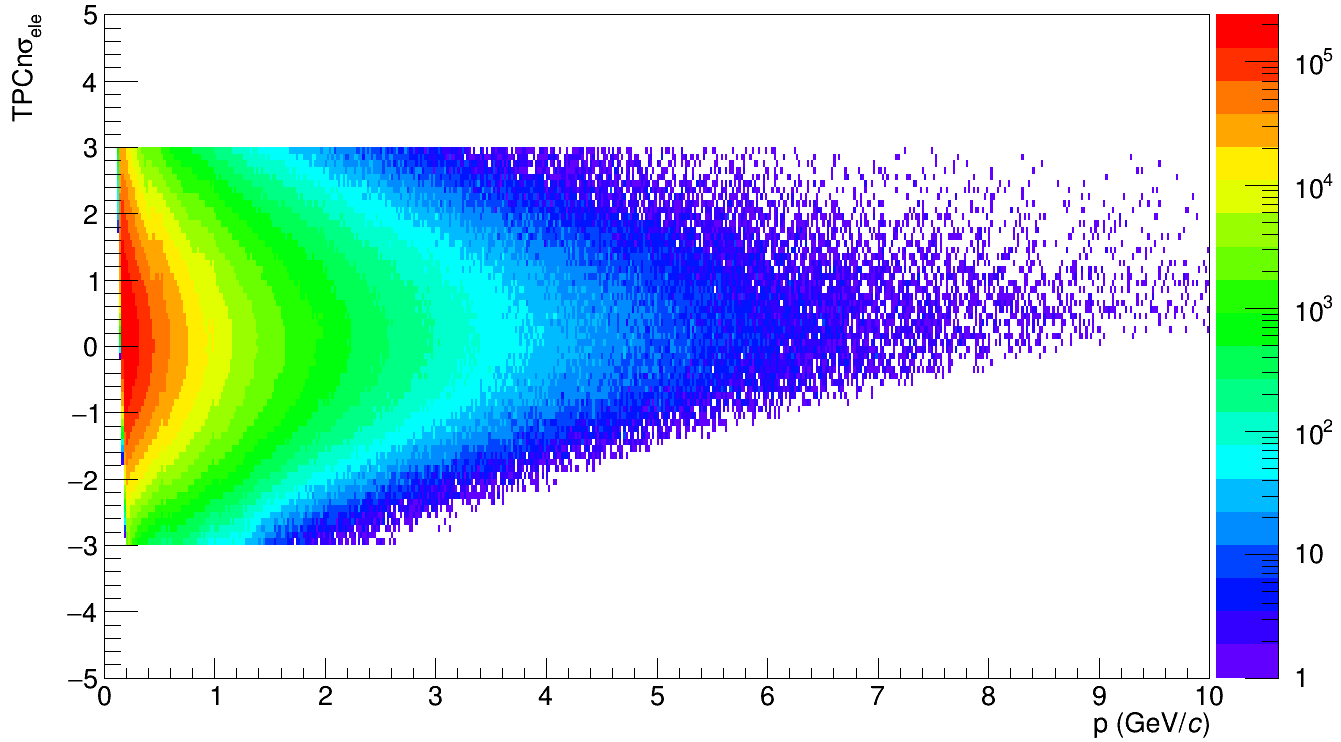
\includegraphics[width=0.98\linewidth]{Figures/V0cuts/tpcnsigmaeleneg.png}
\caption{$n\sigma_e$ versus $p$ plot for the assumption of an electron}
\label{fig:V0tpcele}
\end{subfigure} \hspace{0.1cm}
\begin{subfigure}[t]{.5\linewidth}
\centering
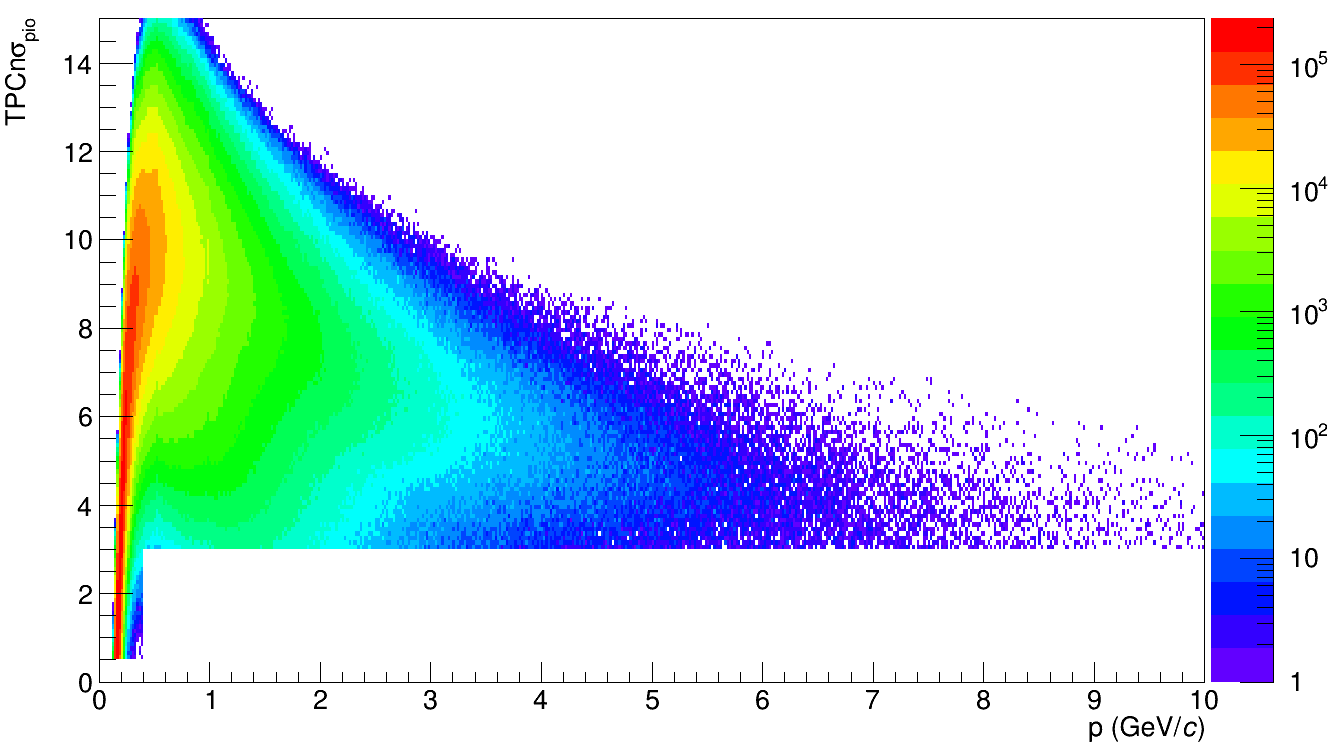
\includegraphics[width=0.98\linewidth]{Figures/V0cuts/tpcnsigmapioneg.png}
\caption{$n\sigma_{\pi}$ versus $p$ plot for the assumption of a pion}
\label{fig:V0tpcpio}
\end{subfigure}
\caption{The specific energy loss of the particles in the TPC expressed in terms of the $n\sigma$ discrimination variable plotted against the particle momentum, here only shown for the negative particles; the colour scale shows the number of counts}
\label{fig:V0tpc}
\end{figure}
After the track cuts we have a basic selection of tracks in the detector. Now, we can start looking for the final products of our decay channel, i.e. the $\pi^0$ and the photon. Since the pion also decays into photons in 99\% of cases, we only have to find photons and then later find out which of them come from pion decays. To find the photons we use the so-called V$^0$ finder of ALICE which finds all decays in the detector which come from a neutral particle and then decay into one positive and one negative particle in a V-like decay, hence the name. In the data all of the V$^0$ candidates are flagged and can be looped over. We can then apply cuts to these V$^0$s to get a good selection of photons. \\
\renewcommand{\arraystretch}{1.3}
\begin{table}[t]
\centering{
\begin{tabular}{@{} ll @{}}
  \toprule			
  V$^0$ Cut & Cut Range \\ \midrule
  pseudorapidity of CP &  $|\eta_{\text{conv}}| < 0.9$ \\ 
  $Z$ coordinate of CP &  $|Z_{\text{conv}}| < 240$ cm \\ 
  radius of CP  &  $5 \ \text{cm} \ < R_{\text{conv}} < 180$ cm \\ 
  line cut  &  $R_{\text{conv}} > |Z_{\text{conv}}| \cdot f \left(\eta_{\text{max}} \right) - Z_0 $\\
  & with $Z_0 = 7$ cm and $\eta_{\text{max}} = 0.9$ \\ 
 $\Psi_{\text{pair}}$ angle  &  $|\Psi_{\text{pair}}| < 0.1$ \\ 
 cosine of pointing angle  &  $\text{cos} \left( \text{pointing angle} \right) > 0.85$ \\ 
 $\chi^2$ of Kalman filter  &  $\chi^2 < 30$ \\
 like-sign cut & reject V$^0$s with like-sign charged legs \\
elliptical cut in Armenteros- \qquad \ \ &  $q_T < q_{T,\text{max}} \cdot \sqrt{1- \alpha^2/\alpha_{\text{max}}^2}$ \\ 
 Podolanski plot &  with $q_{T,\text{max}} = 0.05$ GeV/c, $\alpha_{\text{max}} = 0.95$ \\
  \bottomrule
\end{tabular}
}
\caption{V$^0$ cuts used in the analysis; CP $\widehat{=}$ Conversion Point; $f \left(\eta_{\text{max}} \right)$ is defined in equation \ref{eqn:slope}}
\label{tab:pi0gammaV0cuts}
\end{table}
\renewcommand{\arraystretch}{1.0}
First, we apply some geometrical cuts to only get V$^0$ which are in the acceptance of our detector. The geometrical cuts are the first four cuts in table \ref{tab:pi0gammaV0cuts}. The cut on the pseudorapidity and the $Z$ coordinate of the conversion point makes sure that the conversion happened within the acceptance of our detector. For the radius of the conversion point we have a lower and an upper cut. The lower cut is used to suppress track pairs coming from the primary vertex that might mimic conversions, e.g. lepton pairs from Dalitz decays. The upper cut is used to get rid of conversions which happen late in the TPC. These conversion can't be tracked properly either because the coverage of the legs of the V$^0$ in the TPC is too small. Finally, we also apply a line cute. As the name suggests the line cut rejects all of the conversions that happen below a line in the $ZR$ plane which happen below a line with the slope
\begin{equation}
\label{eqn:slope}
f \left(\eta_{\text{max}} \right) = \text{tan} \left( 2 \ \text{arctan} \left( \text{exp} \left( - \eta_{\text{max}} \right) \right) \right)
\end{equation}
The cut is also a cut to get rid of conversions which happen outside of regions of the detector with a good acceptance. \\
The following cuts in the table are cuts which are related to V$^0$ decays and especially conversions. The $\Psi_{\mathrm{pair}}$ angle is defined by 
\begin{equation}
\label{eqn:psipair}
\Psi_{\text{pair}} = \text{arcsin} \left( \frac{\Delta \theta}{\xi_{\text{pair}}} \right)
\end{equation} 
where $\Delta \theta = \theta_{e^-} - \theta_{e^+}$ is the difference in the polar angle of the daughter tracks of the V$^0$ candidate and 
$\xi_{\text{pair}} = \text{arccos} \left( \frac{\vec{p}_{e^-} \ \cdot \ \vec{p}_{e^+}}{|\vec{p}_{e^-}| \cdot |\vec{p}_{e^+}|} \right)$ 
is the angle between the momentum vectors of the $e^+e^-$ pair. We can understand $\Psi_{\mathrm{pair}}$ better by looking at the invariant mass of a dilapton pair
\begin{equation}
\label{eqn:masspa}
m_{e^+e^-}^2 = 2 E_{e^-} E_{e^+} \cdot \left( 1- \text{cos } \xi_{\text{pair}} \right)
\end{equation}
We have to differ two cases now. If the V$^0$ decay is a photon conversion, the left-hand side is zero up to recoil effects of the nucleus at which the conversion took place. Since the energy of the leptons has to be positive, the angle between the momenta of the leptons also has to be very small. If there was no magnetic field, the leptons would then just fly on straight tracks in the detector. With the field applied along the $z$-axis of the detector this is not the case any more. Since $\vec{F}_L = q \vec{v} \times \vec{B}$, the force on the leptons doesn't have a contribution out of the azimuthal plane. Therefore, the force from the magnetic field can only open the particle tracks in the azimuthal plane but does not have an influence on the polar angle which is only given by the momentum of the mother particle. With this information $\Psi_{\mathrm{pair}}$ should be very close to zero for conversions, because $\Delta\theta$ should be zero for conversions and $\xi_{\mathrm{pair}}$ should only gets contributions from the recoil of the nucleus. \\
In the case of a massive particle the left-hand side is not zero. Therefore the opening angle $\xi_{\mathrm{pair}}$ gets a big contribution according to eqn. \ref{eqn:masspa}. This contribution is not constrained by anything and can therefore also be in the polar direction. Therefore according to \ref{eqn:psipair}, we have a non-zero value for $\Psi_{\mathrm{pair}}$. \\
$\Psi_{\mathrm{pair}}$ can be understood as the angle between the plane that is orthogonal to the magnetic field and the plane that is spanned by the momenta of the leptons. We can therefore use this parameter to distinguish the decay of massless (i.e. photons) from massive V$^0$s. \\
\begin{sidewaysfigure}[p!]
\centering
\begin{subfigure}[h]{.4\linewidth}
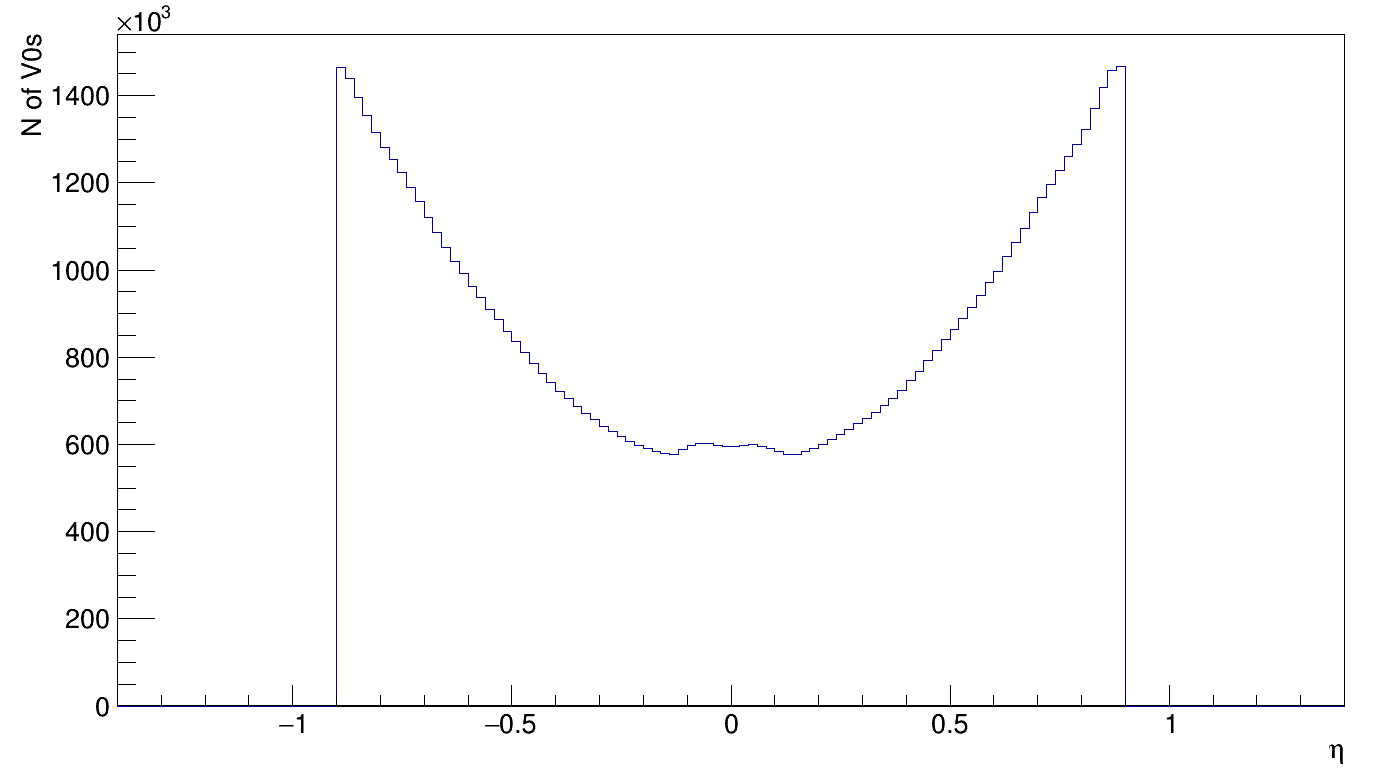
\includegraphics[width=1.0\linewidth]{Figures/V0cuts/V0eta.png}
\caption{Pseudorapidity of the V$^0$ candidate plotted against the number of counts}
\label{fig:V0eta}
\end{subfigure}\hspace{1cm}%
\begin{subfigure}[h]{.4\linewidth}
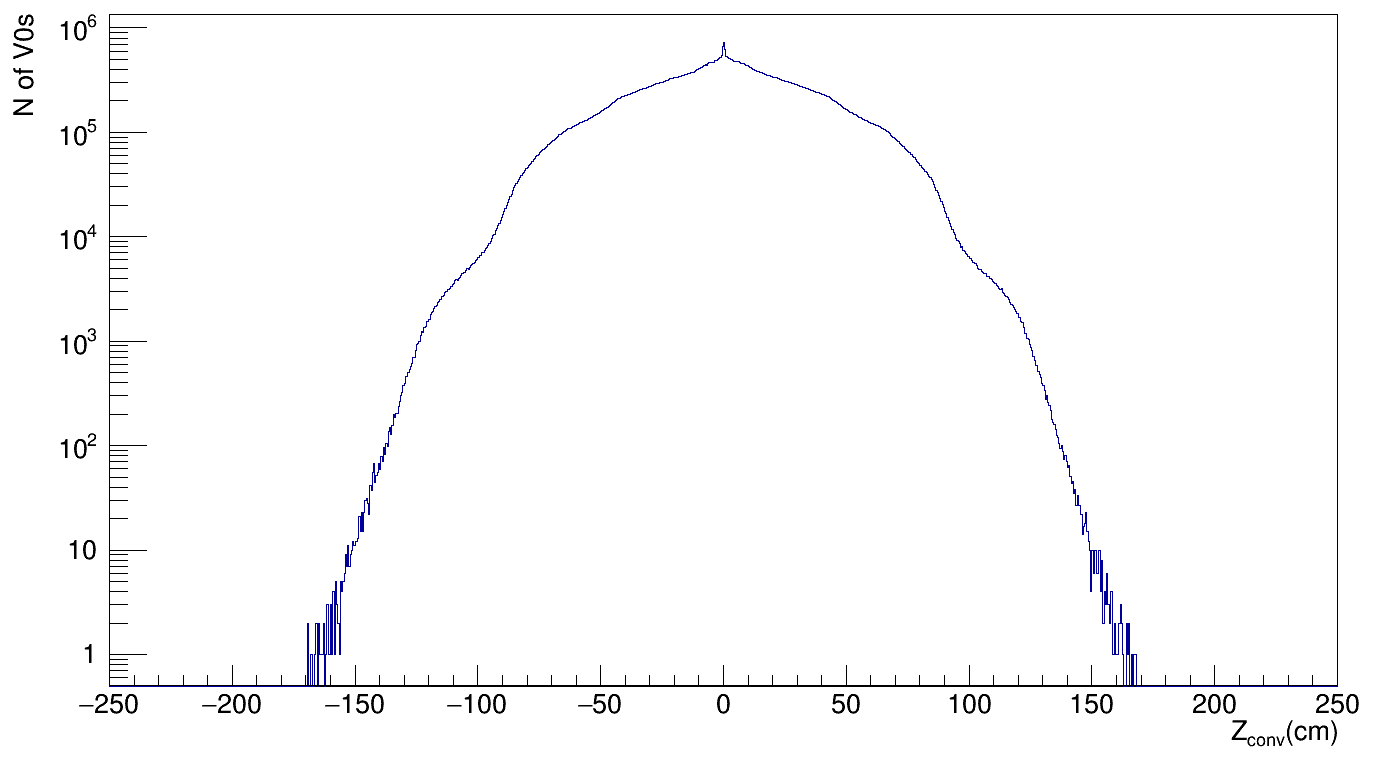
\includegraphics[width=1.0\linewidth]{Figures/V0cuts/V0Z.png}
\caption{$Z$ coordinate of the conversion point plotted against the number of counts}
\label{fig:V0Z}
\end{subfigure}

\vspace{0.7cm}

\begin{subfigure}[h]{.4\linewidth}
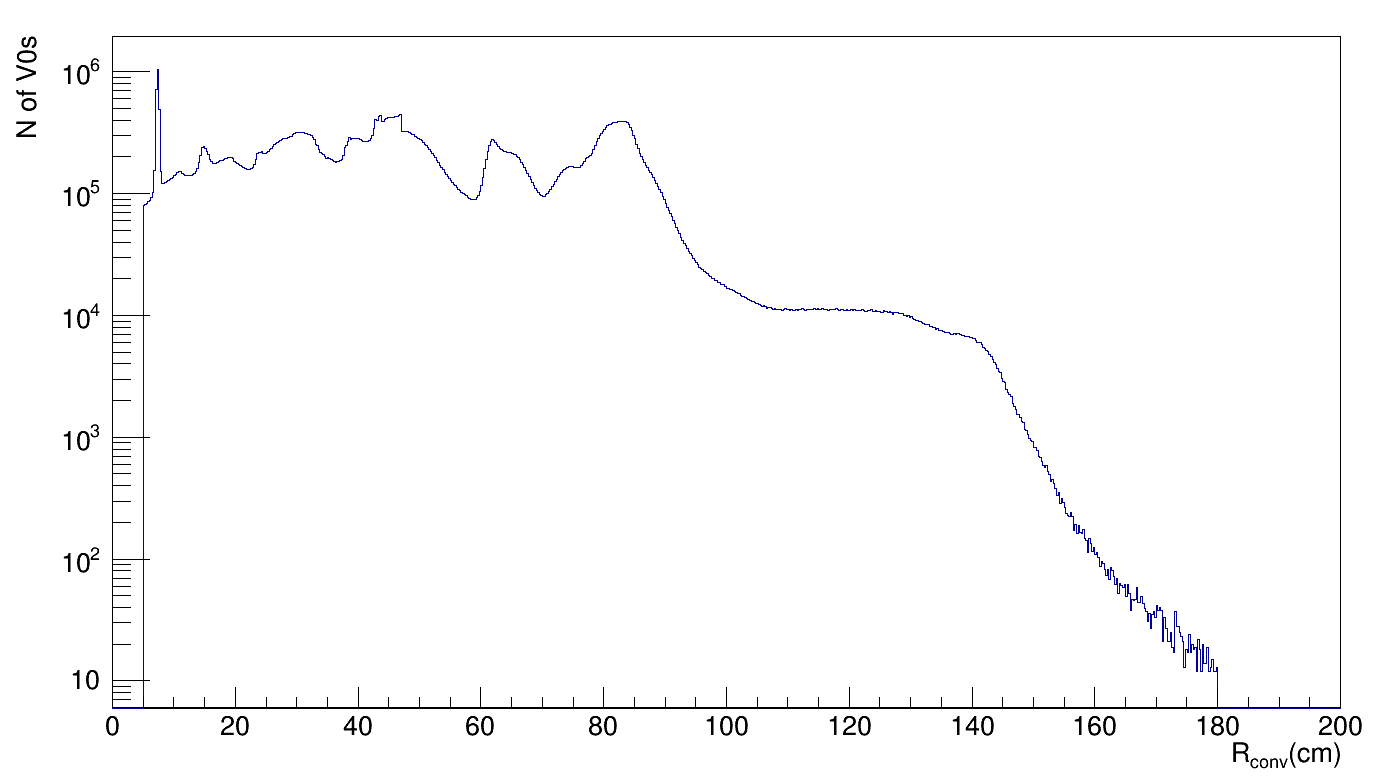
\includegraphics[width=1.0\linewidth]{Figures/V0cuts/V0radius.png}
\caption{\centering{Radius of the conversion point plotted against the number of counts}}
\label{fig:V0R}
\end{subfigure}\hspace{1cm}%
\begin{subfigure}[h]{.4\linewidth}
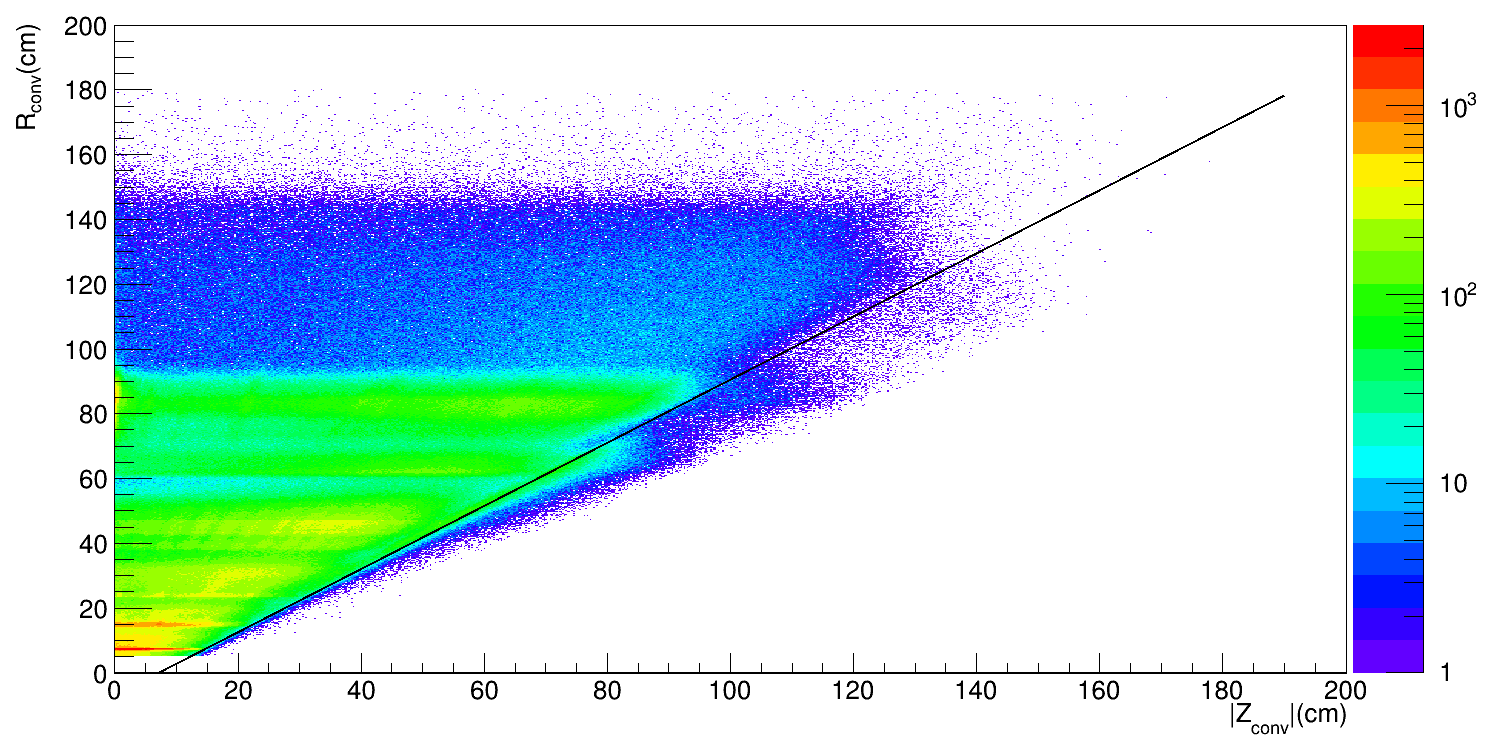
\includegraphics[width=1.0\linewidth]{Figures/V0cuts/V0RvsZwlinecut.png}
\caption{$Z$ coordinate of the conversion point plotted against the radius of the conversion point; the line shows the line cut defined in table \ref{tab:V0cuts} and the colour scale shows the number of counts}
\label{fig:V0linecut}
\end{subfigure}
\vspace{0.5cm}
\caption{Plots of the geometric V$^0$ cuts as they were used in this analysis}
\label{fig:V0cuts}
\end{sidewaysfigure}

\begin{sidewaysfigure}[p!]
\centering
\begin{subfigure}[h]{.4\linewidth}
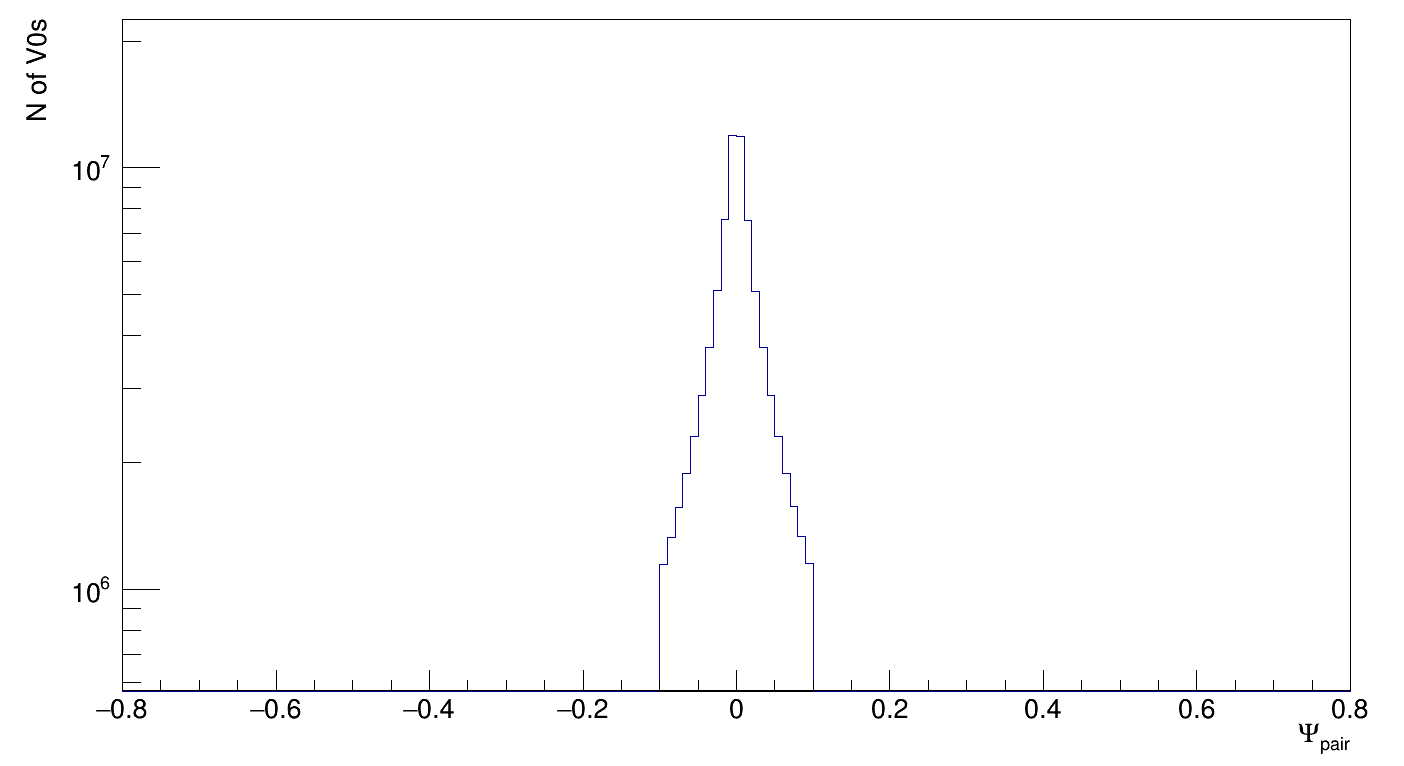
\includegraphics[width=1.0\linewidth]{Figures/V0cuts/V0psipair.png}
\caption{$\Psi_{pair}$ angle of the V$^0$ candidate plotted against the counts}
\label{fig:V0psipair}
\end{subfigure}\hspace{1cm}%
\begin{subfigure}[h]{.4\linewidth}
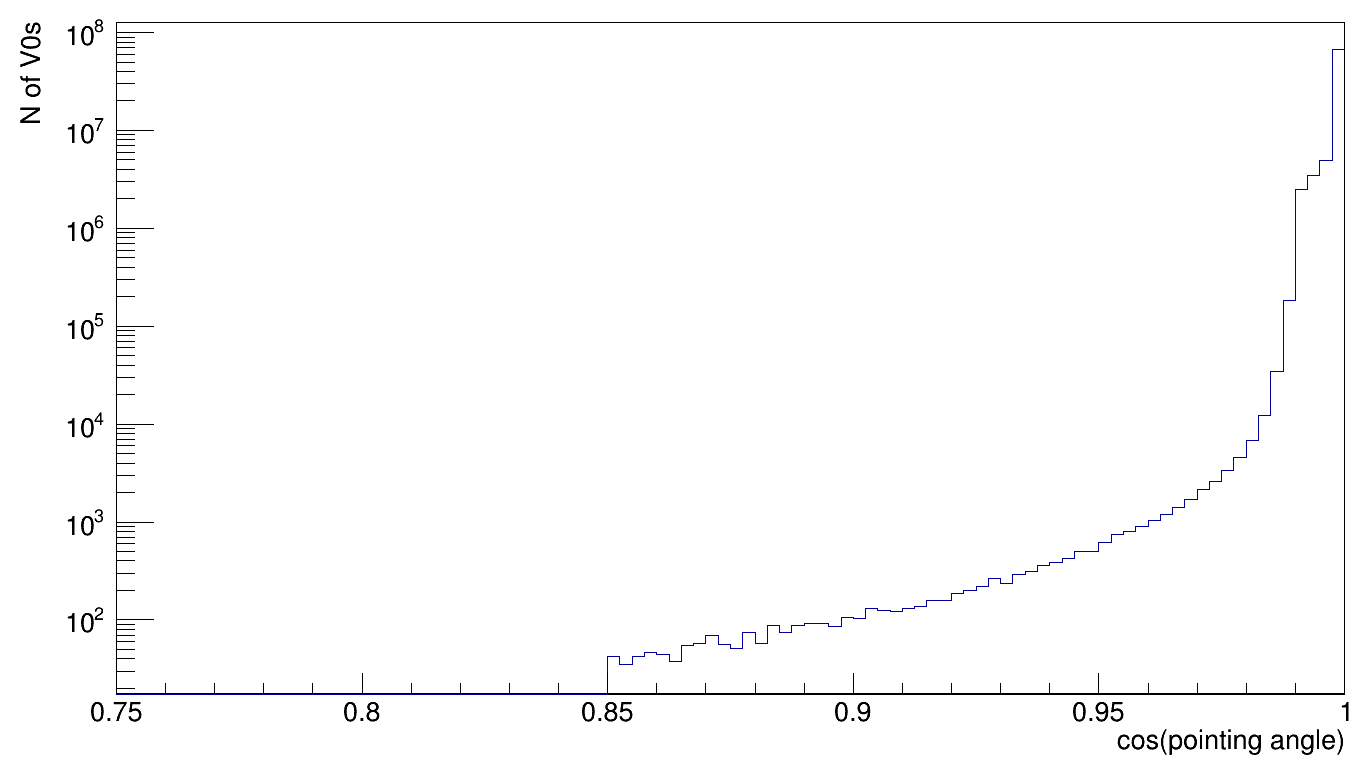
\includegraphics[width=1.0\linewidth]{Figures/V0cuts/V0cospa.png}
\caption{cos(pointing angle) of the legs of the V$^0$ plotted against the counts}
\label{fig:V0cospa}
\end{subfigure}

\vspace{0.7cm}

\begin{subfigure}[h]{.4\linewidth}
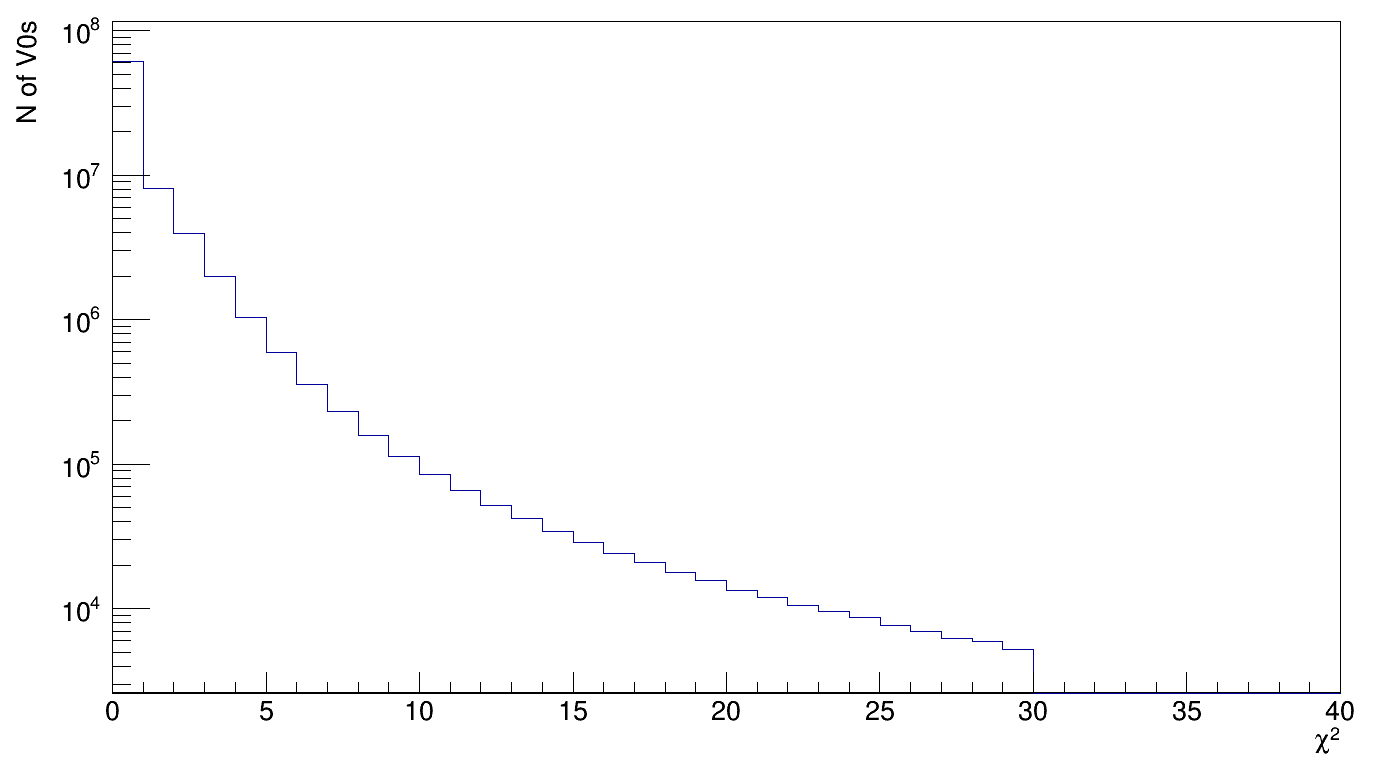
\includegraphics[width=1.0\textwidth]{Figures/V0cuts/V0chi2.png}
\caption{$\chi^2$ of the Kalman filtering method of tracks which form the V$^0$ plotted against the counts}
\label{fig:V0chi2}
\end{subfigure}\hspace{1cm}%
\begin{subfigure}[h]{.4\linewidth}
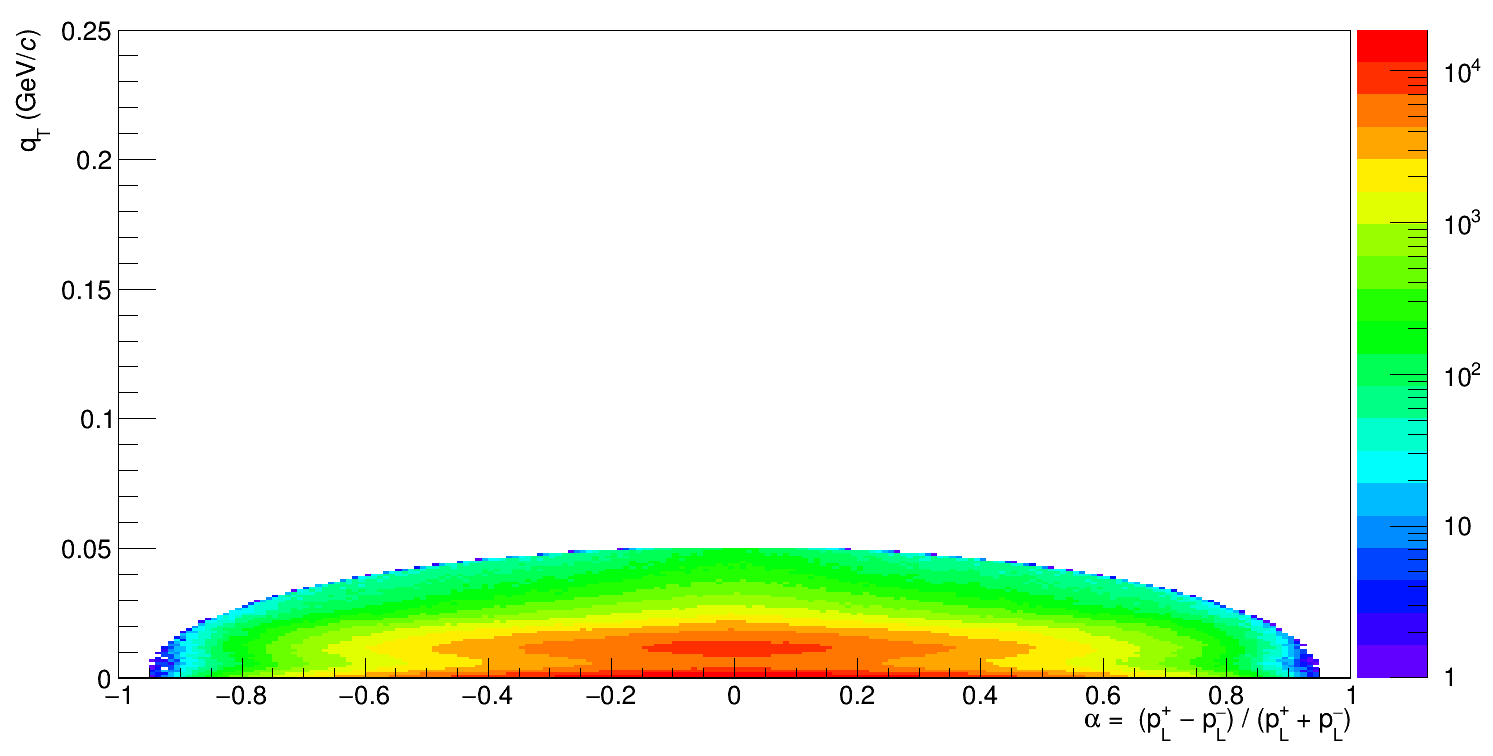
\includegraphics[width=1.0\linewidth]{Figures/V0cuts/armpod.png}
\caption{Armenteros-Podolanski plot with the cut selecting the photons from the V$^0$ candidates}
\label{fig:V0armpod}
\end{subfigure}
\vspace{0.5cm}
\caption{Plots of the further V$^0$ cuts as they were used in this analysis}
\label{fig:V0cuts}
\end{sidewaysfigure} 
The next cut is a cut on the pointing angle which is the angle between the line defined by the V$^0$ legs pointing back to the V$^0$ vertex and the line which is defined by connecting the V$^0$ vertex to the primary vertex. If the V$^0$ vertex under consideration really comes from a V$^0$ decay the legs obviously should point back to the mother momentum and therefore the primary vertex, so the pointing angle should be zero. \\
We also used a cut on the $\chi^2$ value of the Kalman filter which is used during the reconstruction procedure of the V$^0$ vertex. We chose the value such that we have a good selection of V$^0$s but simultaneously also do not lose too much statistics. \\
The like-sign cute was added to get rid of false V$^0$s where the leptons have the same charge. The amount of V$^0$s rejected by this cut is quite low but since these decays are definitely no real V$^0$ decays it it still worth it to get rid of them. \\
The last V$^0$ cut is a cut in the so-called Armenteros-Podolanski plot. In the Armenteros-Podolanski plot, the longitudinal momentum asymmetry of the daughter particles
\begin{equation}
\alpha = \frac{p_L^{+} - p_L^{-}}{p_L^{+} + p_L^{-}}
\end{equation}
is plotted against the transverse momentum of one of the daughter particles with respect to the momentum of the V$^0$ candidate
\begin{equation}
q_T = \frac{|\vec{p}^{-} \times \vec{p}_{V^0}|}{|\vec{p}_{V^0}|}
\end{equation}
Looking again at eqn. \ref{eqn:masspa}, we know that $\xi_{\mathrm{pair}}$ must be zero. Therefore, photon conversions can not contribute to the transverse momentum of the dielectron pair because they fly in the same direction after the conversion. Thus, we expect photon conversions to be at the bottom of the Armenteros-Podolanksi plot. The only small contribution to $q_T$ comes again from recoil effects from the nucleus. That is why we used an elliptical cut around the bottom of the plot to cut off the ellipses from massive V$^0$ decays and get a good selection of photon conversions. \\
The cuts which were described up to this point are heavily inspired or completely adopted from other similar analyses performed in the ALICE Collaboration \cite{ananote1, ananote2}. The analysis notes review works using the conversion method to measure the properties of neutral mesons and to determine the material budget of the ALICE detector. \\
\begin{sidewaysfigure}[p!]
\centering
\begin{subfigure}[h]{.4\linewidth}
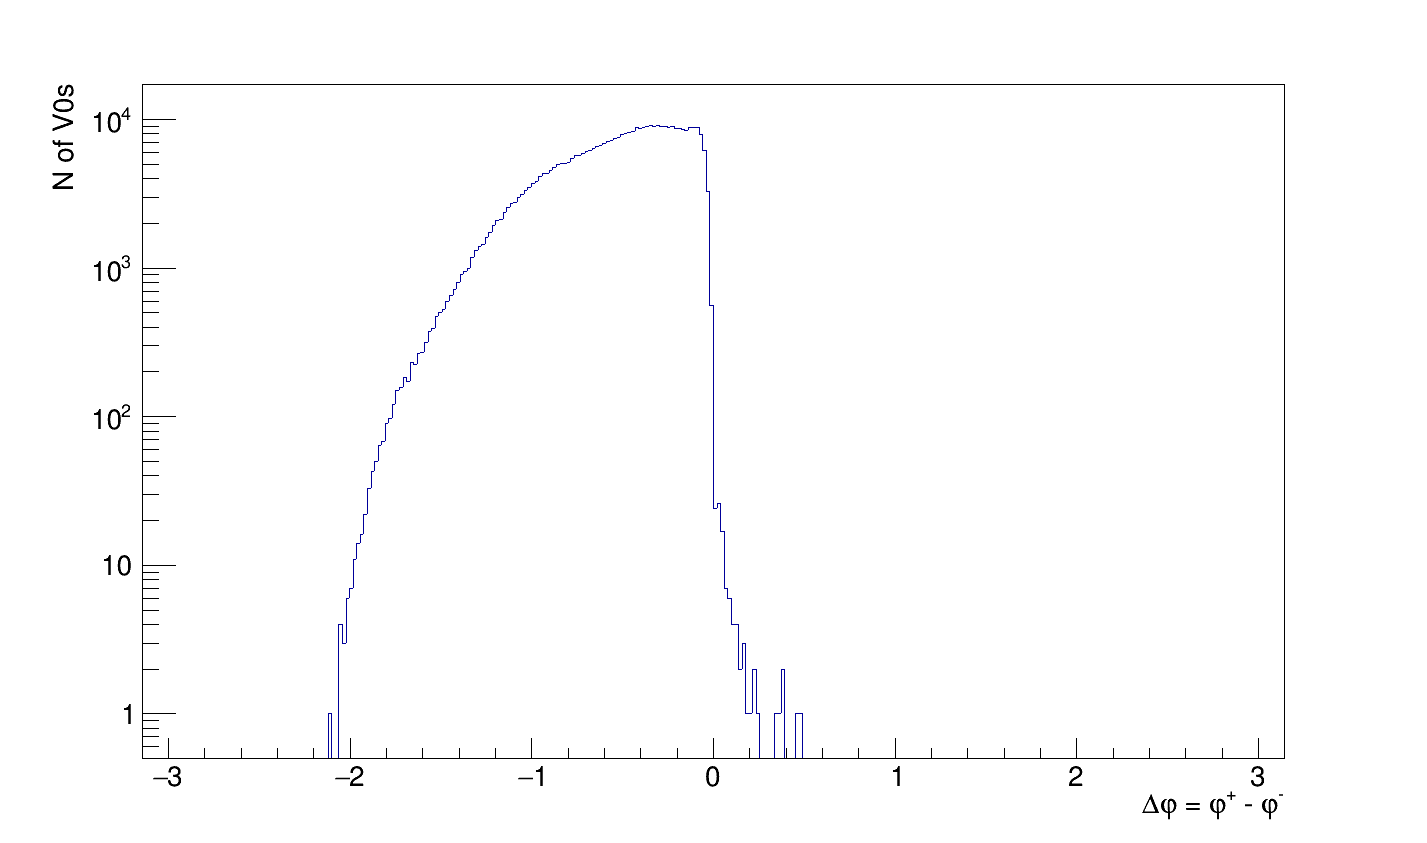
\includegraphics[width=1.0\linewidth]{Figures/additionalV0cuts/DeltaPhi.png}
\caption{Difference of azimuthal angle $\Delta\phi$ of V$^0$ legs plotted against number of counts}
\label{fig:DPhi}
\end{subfigure}\hspace{1cm}%
\begin{subfigure}[h]{.4\linewidth}
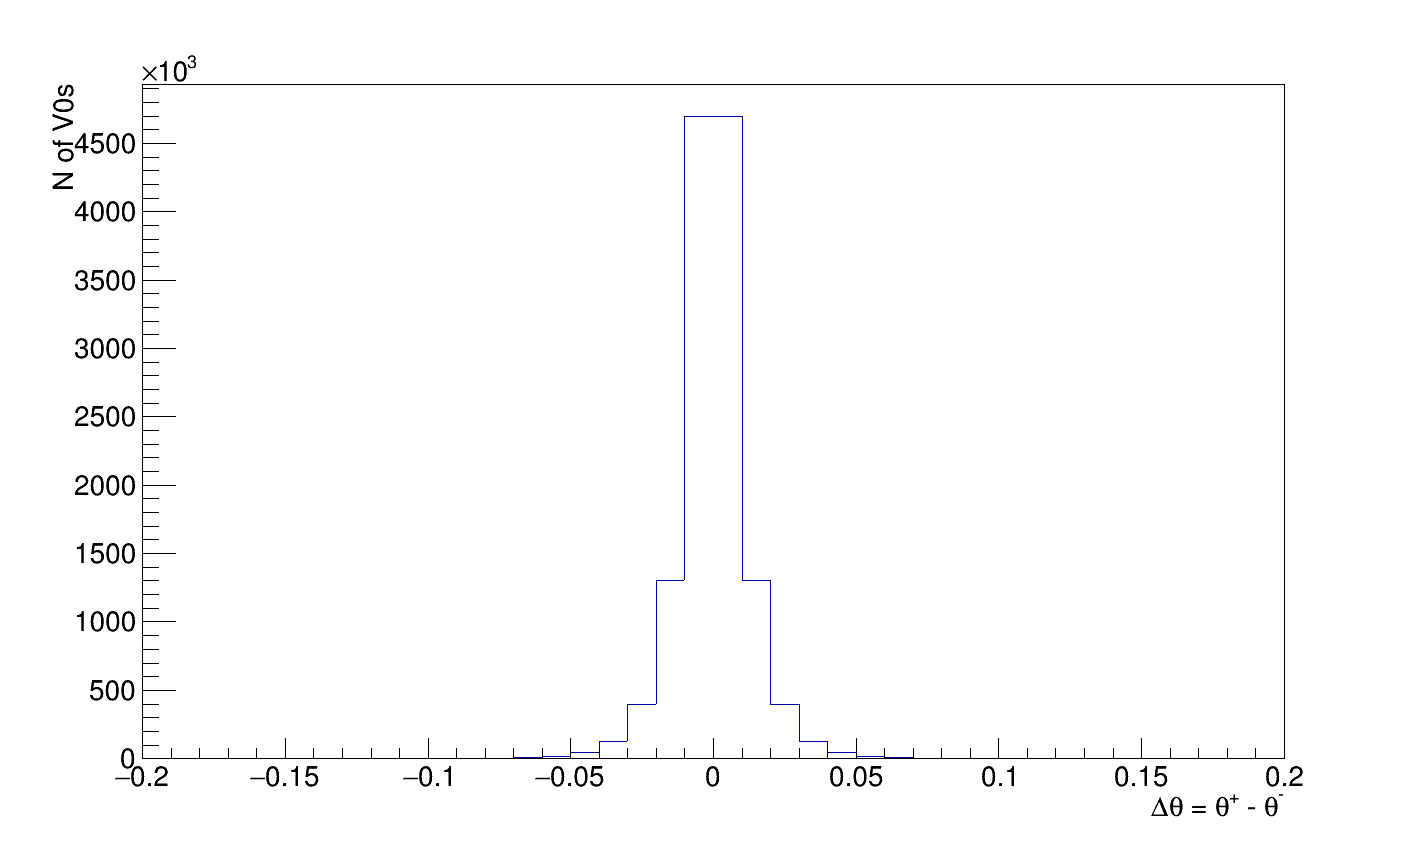
\includegraphics[width=1.0\linewidth]{Figures/additionalV0cuts/DeltaTheta.png}
\caption{Difference of polar angle $\Delta\theta$ of V$^0$ legs plotted against number of counts}
\label{fig:DTheta}
\end{subfigure}

\vspace{0.7cm}

\begin{subfigure}[h]{.4\linewidth}
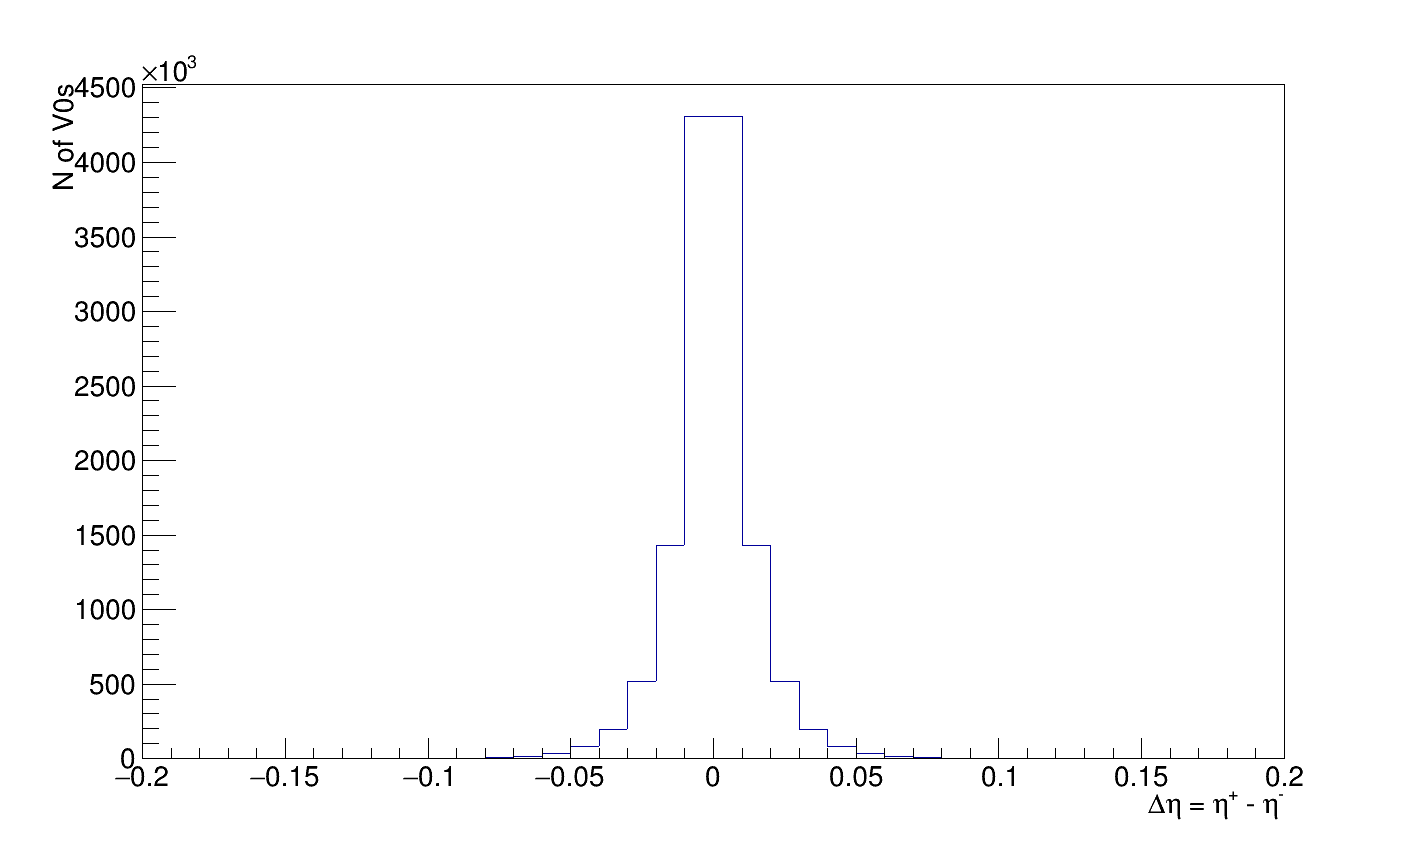
\includegraphics[width=1.0\linewidth]{Figures/additionalV0cuts/DeltaEta.png}
\caption{\centering{Difference of pseudorapidity $\Delta\eta$ of V$^0$ legs plotted against number of counts}}
\label{fig:DEta}
\end{subfigure}\hspace{1cm}%
\begin{subfigure}[h]{.4\linewidth}
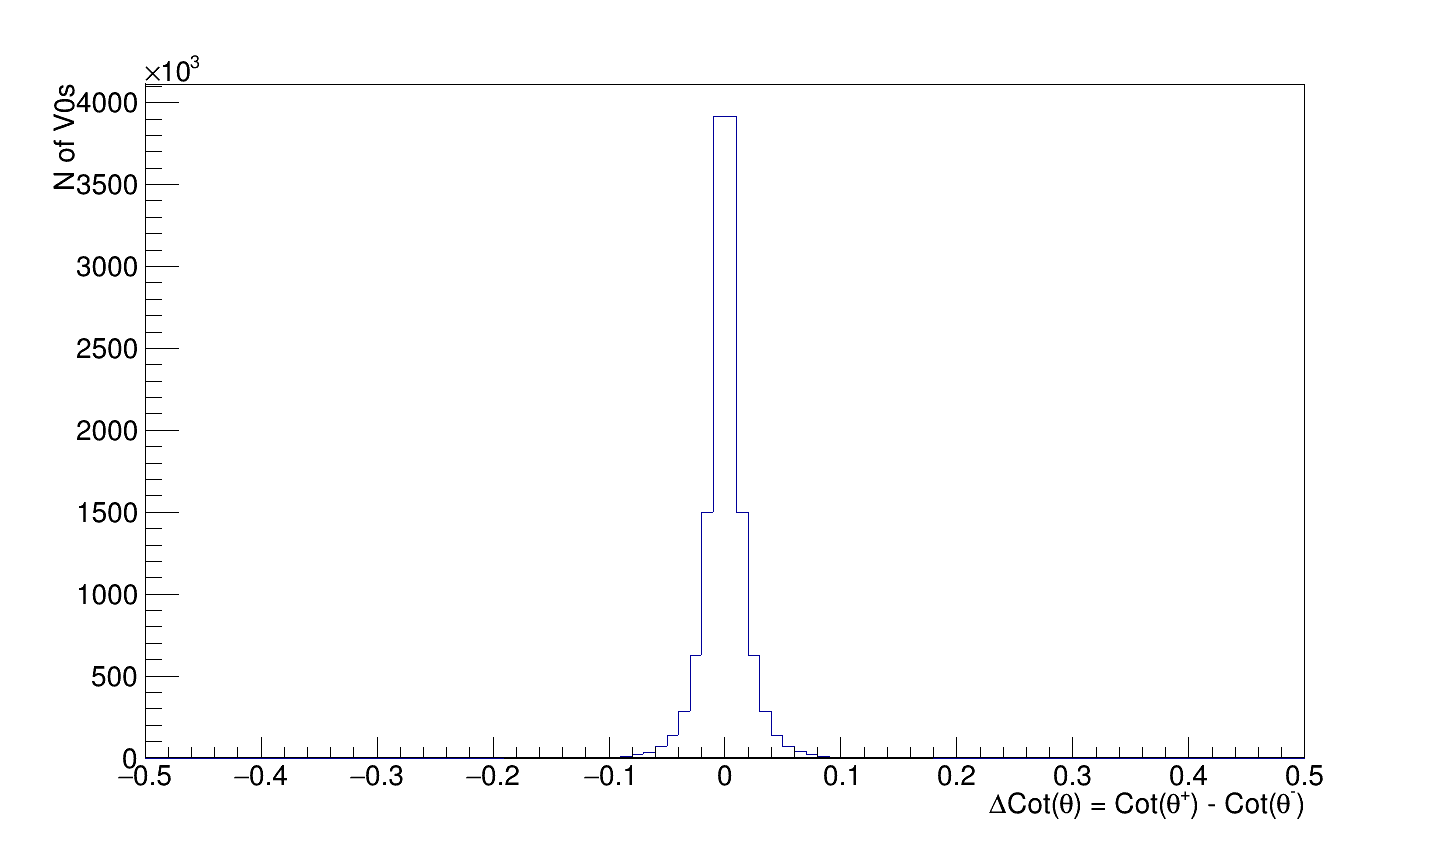
\includegraphics[width=1.0\linewidth]{Figures/additionalV0cuts/DeltaCotTheta.png}
\caption{Difference of Cotangent of polar angle $\mathrm{Cot}\Delta\theta$ of V$^0$ legs plotted against number of counts}
\label{fig:DCotTheta}
\end{subfigure}
\vspace{0.5cm}
\caption{Plots of further geometric V$^0$ cuts which were not used in this analysis}
\label{fig:addV0cuts}
\end{sidewaysfigure}
We also considered a few other cuts which can be found in figure \ref{fig:addV0cuts}. The cuts you can see there also exploit properties of conversions. The first figure shows the difference of the azimuthal angle $\Delta\phi$ between the V$^0$ legs which should be negative for conversions for a negative magnetic field. But the abundance of V$^0$s with positive $\Delta\phi$ is so small that the effect of applying the cut would not even be visible. Therefore, we did cut on $\Delta\phi$. \\
The second plot shows the difference of the polar angle $\Delta\theta$ between the V$^0$ legs. As already discussed above this should be zero because converting photons cannot naturally contribute to the opening angle of their daughters and the magnetic field only acts in the azimuthal plane and therefore also cannot change the polar angle of the leptons. Since the distribution around zero is quite sharp we also did not cut on $\Delta\theta$. \\
The other two plots show the distribution of the difference of the pseudorapidity and the difference of the cotangent of the polar angle between the V$^0$ legs. Since both the pseudorapidity $\eta = -\log\tan\frac{\theta}{2}$ and $\mathrm{cot}\theta$ are continuous functions of $\theta$ and the $\theta$ distribution was already sharp around zero, we also do not expect a huge difference in these distributions. Thus, we also did not cut on $\Delta\eta$ and $\Delta\mathrm{cot}\theta$. \\
The last check we also considered was if the reconstructed radii of the helices of the V$^0$ legs is compatible with the coordinates of the legs. For that we calculated the difference of the helix centre from the coordinates of the legs. Then we subtracted the radius of both helices. If the difference is zero the reconstruction worked well. The distribution of the distance between the helices can be found in figure \ref{fig:helixdist}. The distribution looks reasonable with a trend of slightly overestimating the curvature radius. But with the cut we would not gain a lot. The cut is also hard to implement in an AOD analysis and it would be too time consuming to use ESDs with the amount of data we used. So we did not use the cut. \\
\begin{figure}[t]
	\centering
	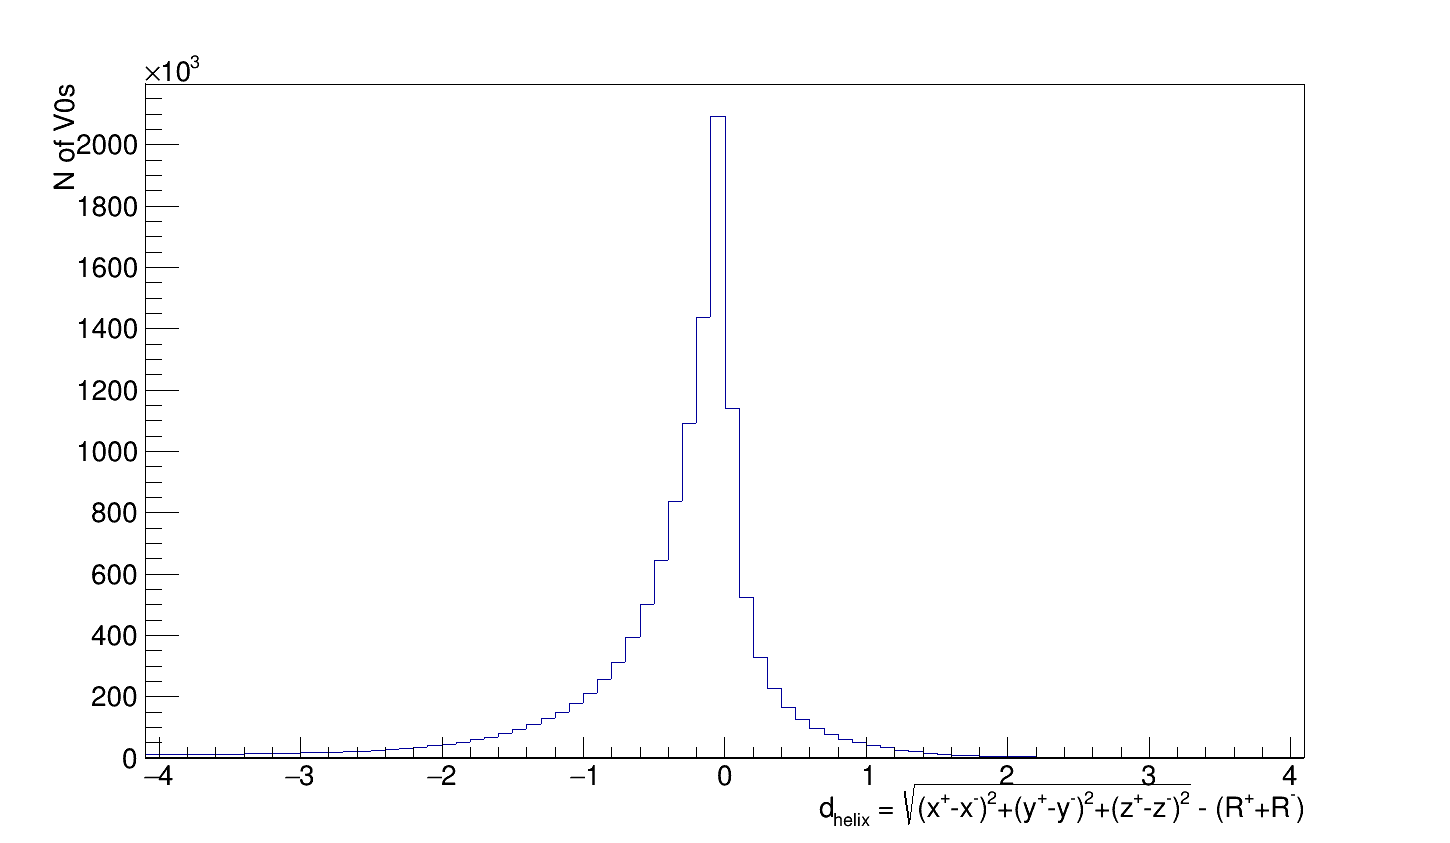
\includegraphics[width=0.8\linewidth]{Figures/additionalV0cuts/helixdist.png}
	\caption{Distance between helices of V$^0$ legs defined by radius which was obtained during the reconstruction process of the tracks}
	\label{fig:helixdist}
\end{figure}

\subsubsection{Analysis with Calorimeters}
For the calorimeter analysis all of the calorimeters in ALICE where used. Namely, the Photon Spectrometer (PHOS) and the electromagnetic calorimeter (EMCAL) also including the Di-jet Calorimeter (DCAL). Since the DCAL is just an addendum to the EMCAL which was added later to be able to reconstruct jets better we will refer to EMCAL+DCAL as EMCAL for short. \\
For the calorimeter analysis we used the same event preselection as for the PCM analysis. Then, specific calorimeter cuts were applied which can be found in table \ref{tab:calocuts}. The first cut requires the number of clusters in an event to be bigger than two which makes sure that at least one decay happened in the event and was recorded with either the EMCAL or the PHOS. Then we applied shower shape cuts to the particle showers for both EMCAL and PHOS. On approach to differentiate between different shower shapes is to use a covariance matrix \cite{CaloCovMat}. The covariance matrix is defined by
\begin{equation}
M_{ij} = \left( x_i(E) - \bar{x}_i((E) \right)\left( x_j(E) - \bar{x}_j((E) \right)
\end{equation}
where $x_i(E)$ is the total pulse height observed in one calorimeter block at energy $E$ and $\bar{x}_i((E)$ is the expected pulse height that can be obtained from simulations or a study of the response of the detector with a test beam at different energies. The diagonal elements of the matrix give the variance of the pulse height in each calorimeter block while the off-diagonal elements give the correlation between the calorimeter blocks. We can also define a $\chi^2$ function with help of the covariance matrix as follows
\begin{equation}
\chi^2(E) = X_i(E) M_{ij}^{-1}(E) X_j(E)
\end{equation}
where $X_i(E) = x_i(E) - \bar{x}_i((E)$.
In the EMCAL the shower shape cut is applied by requiring that the eigenvalue of the covariance matrix lies within a lower and an upper bound. This makes sure we select particle showers coming from photons which have a certain shower shape that can be differentiated from other particles. For the PHOS we also apply a cut on the shower shape by cutting on the $\chi^2$ value obtained from the covariance matrix. \\
\\
\\
time of flight?? \\
\\
\\
We can also improve the neutral cluster detection in PHOS with help of a charged particle veto which is provided by a dedicated detector. If there's a hit of a charged particle in the CPV detector it can be matched to the clusters in the calorimeter and the cluster corresponding to the charged particle can be removed. \\
Besides the CPV matching capability we can also try to match the other tracks in the detector to match them to clusters which come from charged particles. \\
\\
\\
In the PHOS this is done by .. z coordinate normalized with respect to what??
\\
\\
In the EMCAL the matching is done by comparing the pseudorapidity $\eta_{\mathrm{proj}}$ and azimuthal angle $\phi_{\mathrm{proj}}$ of the charged particle track projected on the surface of the PHOS with the pseudorapidity $\eta_{\mathrm{EMCAL}}$ and azimuthal angle $\phi_{\mathrm{EMCAL}}$ of the cluster in the EMCAL. If they coincide within a certain accuracy, the cluster is removed from the analysis. \\
Finally, we also apply energy cuts to both the PHOS and the EMCAL. The lower cut is used to get rid of low-energy noise and the high cut is used to get rid of anomalous events at extremely high energies.

include calo plots:
phi-eta distribution, energy cut, $\chi^2$ cuts?

write about correction task


\renewcommand{\arraystretch}{1.3}
\begin{table}[t]
\centering{
\begin{tabular}{@{} ll @{}}
  \toprule		
  Calorimeter Cut \qquad & \qquad Cut Range \\ \midrule
  Number of Clusters \qquad & \qquad $N_{\mathrm{Cluster}} \geq 2$ \\ 
  Shower Shape EMCAL \qquad & \qquad $ 0.1 < \lambda < 0.366$ \\ 
  Cluster $\chi^2$ PHOS \qquad & \qquad $\chi^2 < 6.25$ \\
  Time Of Flight \qquad & \qquad $t_{\mathrm{TOF}} < 12.5$ ns \\
  Charged Particle Veto \qquad & \qquad TRUE \\
  PHOS Track Matching \qquad & \qquad $\sqrt{\Delta\phi^2 + \Delta z^2} < 10$  \\ 
  EMCAL Track Matching \qquad & \qquad  $\sqrt{\left(\eta_{\mathrm{proj}}-\eta_{\mathrm{EMCAL}}\right)^2 + \left(\phi_{\mathrm{proj}}-\phi_{\mathrm{EMCAL}}\right)^2} < 0.05$ \\ 
  EMCAL Energy Cut \qquad & \qquad $0.7 \ \mathrm{GeV} \ < E_{\mathrm{EMCAL}} < 100$ GeV \\
  PHOS Energy Cut \qquad & \qquad $0.2 \ \mathrm{GeV} \ < E_{\mathrm{PHOS}} < 100$ GeV \\
  \bottomrule 
\end{tabular}
}
\caption{EMCAL AND PHOS cuts for the $a_1 \rightarrow \pi^0\pi^{+}\pi^{-}$ decay}
\label{tab:calocuts}
\end{table}
\renewcommand{\arraystretch}{1.0}



\subsection{$a_1 \rightarrow \pi^0\pi^{+}\pi^{-}$ Analysis}
For the analysis of the 3$\pi$ final state we used the same event selection as for the other analysis. Since we also reconstructed the neutral pion with the conversion of the photons it decays into, we also used the same cuts as above (c.f. table \ref{tab:pi0gammacuts} and \ref{tab:pi0gammaV0cuts}) to find the electron tracks and then the converted photons in the detector. For the charge pions we had to do a bit more worked because they are the most abundant species in a pp collision and we wanted to make sure to get a very clean selection of pions. \\
For the charged pions we used the cuts which are known as the 2011 standard ITS-TPC track cuts in ALICE. They can be found in table \ref{tab:3pipiocuts}. \\
The first cut is a cut on $p_T$ which was also used for the electrons to get rid of low momentum particles which cannot be tracked properly. Unlike in the case of electron tracks where the electrons are no final state particles, we now have apply all of the cuts directly to the charged pions and not to some mother particle like the photon candidates before. Therefore we also apply a pseudorapity cut to the charged pion tracks to make sure that they lie within the acceptance of our detector. Then as in the electron case we also apply TPC cluster cuts. Here they are more strict since pions are the most abundant species in pp collisions. Apart from the ratio of TPC clusters over all findable TPC clusters we also require the tracks to have crossed at least 70 rows of the TPC to make sure they are recorded properly and don't lie in dead spots of the TPC. We also apply a cut on the $\chi^2$ of the TPC clusters to make sure the tracks were reconstructed properly in most of the cells. Then, we require a refit in the TPC and to the ITS. These refits already happen during the reconstruction of the tracks during the basic event reconstruction. In the ITS refit the tracks from the TPC are fitted to the hits in the ITS to get more track information from the whole detector. In the TPC refit the whole track is refitted from the innermost point in the detector to the TPC to make sure that the we get a good fit for the whole global track without any artefacts like kinks etc. Then we also make assumptions on the behaviour of the distance of closest approach (DCA) to the primary vertex in the $XY$ plane as a function of the track $p_T$ which should be below a certain threshold. Here, low-energy particles are allowed to be farther away from the primary vertex because the tracking does not work as well at low momenta. We also cut on the DCA in the $z$-direction where the transverse momentum of the particle obviously does not matter since the bigger part of the momentum in the $z$-direction comes from pre-collision kinematics. We then also cut on the $\chi^2$ value of the clusters in the ITS and the $\chi^2$ value we obtain from comparing the global track obtained from combining the TPC with the ITS track with the constrained TPC track. As before we also reject tracks with kinks because they correspond to a weak decay topology. We do not require the $\sigma$ to vertex option which when enabled requires the distance from the track to the vertex to be calculated in terms of the standard deviation $\sigma$. \\
For the PID in addition to the TPC we also used the time of flight (TOF) detector here. The TOF detector measures the time of flight through the detector area from which we the particle velocity $\beta$ can be calculated. We can then plot the velocity against the momentum which is mass dependent. Therefore we can identify the particle by making an assumption on the mass. As for the selection for the electrons before we used a cut of 3$\sigma$ for both the TPC and the TOF cut. We did not apply a rejection of other particles since pions are a lot more abundant than other species and we would lose more statistics from cutting out the area where other particles cross the Bethe-Bloch line of the pions than gaining informaation from rejecting the wrong particles in the PID which can also be rejected by other cuts, e.g. by also applying the TOF PID cuts. In fig. \ref{fig:PIDChPio} a plot of the $n\sigma$ variable for the assumption of a pion versus the momentum can be found for the TPC and TOF.
\renewcommand{\arraystretch}{1.3}
\begin{table}[t]
\centering{
\begin{tabular}{@{} ll @{}}
  \toprule		
  Track Cut \qquad & \qquad Cut Range \\ \midrule
  track $p_T$ \qquad & \qquad $p_T > 0.05$ GeV/c \\ 
  track pseudorapidity \qquad & \qquad $|\eta| < 0.8$ \\ 
  TPC clusters \qquad & \qquad $\frac{N_{\text{TPC-Clusters}}}{N_{\text{findable TPC-Clusters}}} > 0.8$ \\
  crossed TPC rows \qquad & \qquad $N_{\mathrm{crossed \ rows}} > 70 $ \\
  TPC cluster $\chi^2$ \qquad & \qquad $\frac{\chi^2}{N_{\mathrm{clusters}}} < 4 $ \\
  require TPC refit \qquad & \qquad TRUE \\ 
  require ITS refit \qquad & \qquad TRUE \\ 
  DCA to vertex $p_T$ dependence \qquad & \qquad $ DCA_{XY} < 0.0105 \ \mathrm{cm} + \frac{0.0350 \ \mathrm{cm}}{\left(\frac{p_T}{\mathrm{GeV}}\right)^{1.1}}$ \\
  DCA z-coord. to vertex \qquad & \qquad $ DCA_Z < 2$ cm \\
  ITS cluster $\chi^2$ \qquad & \qquad $\frac{\chi^2}{N_{\mathrm{clusters}}} < 36 $ \\
  $\chi^2$ constrained vs global track \qquad & \qquad $\chi^2 < 36$ \\ 
  rejection of tracks with kinks \qquad & \qquad TRUE \\ 
  require sigma to vertex \qquad & \qquad FALSE \\ 
  \midrule
  pion selection \qquad & \qquad $|n\sigma_{\pi,TPC}| < 3$ \\ \
 \qquad & \qquad $|n\sigma_{\pi,TOF}| < 3$ \\
  \bottomrule 
\end{tabular}
}
\caption{General track and PID cuts for the pions from the $a_1 \rightarrow \pi^0\pi^{+}\pi^{-}$ decay}
\label{tab:3pipiocuts}
\end{table}
\renewcommand{\arraystretch}{1.0}

\begin{figure}[t]
\begin{subfigure}[b]{0.5\linewidth}
\centering
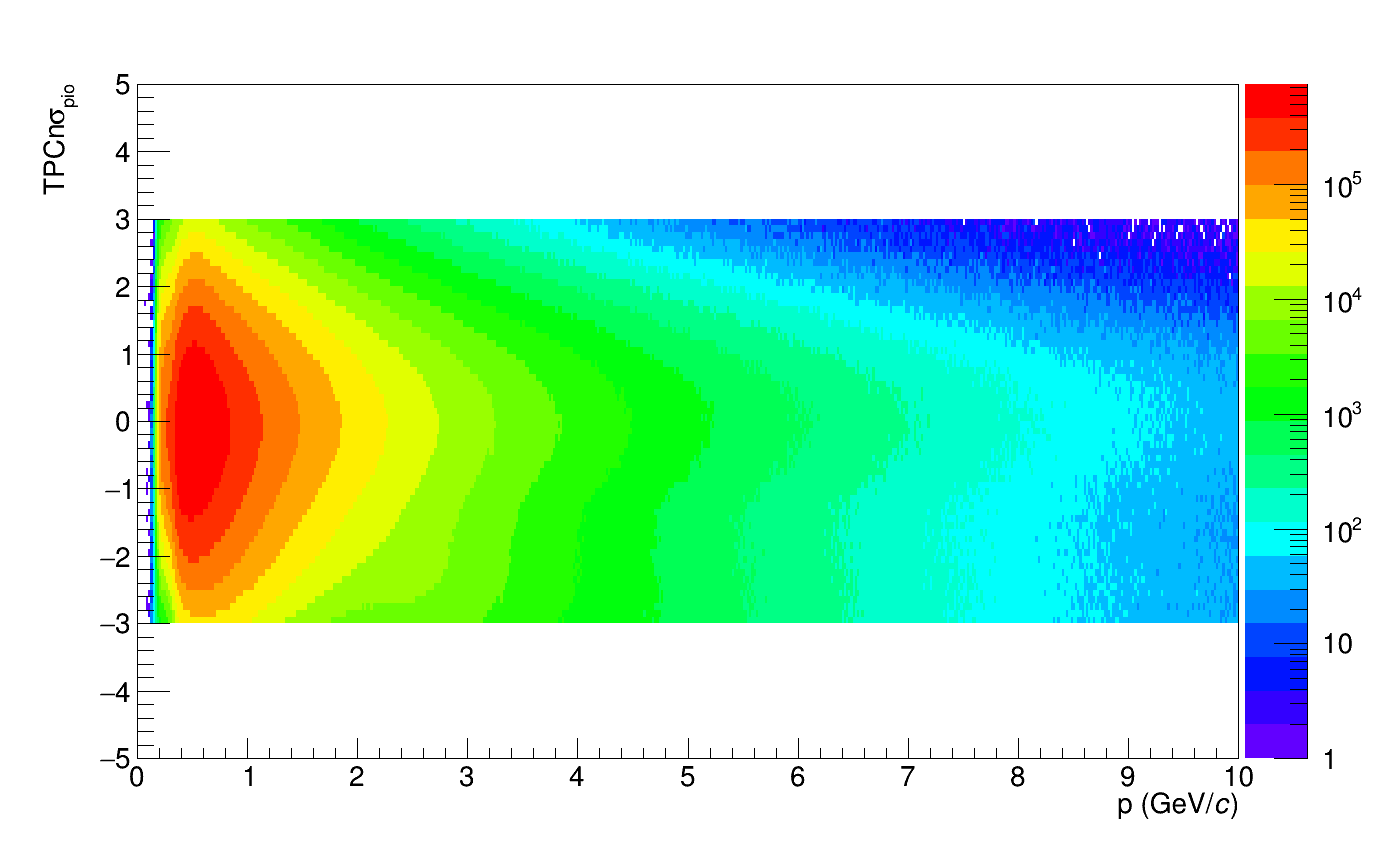
\includegraphics[width=0.98\linewidth]{Figures/ChargedPioCuts/TPCnsigmapioneg.png}
\caption{$n\sigma_{\pi}$ versus $p$ plot for the assumption of a pion in the TPC}
\label{fig:ChpioTPC}
\end{subfigure} \hspace{0.1cm}
\begin{subfigure}[b]{.5\linewidth}
\centering
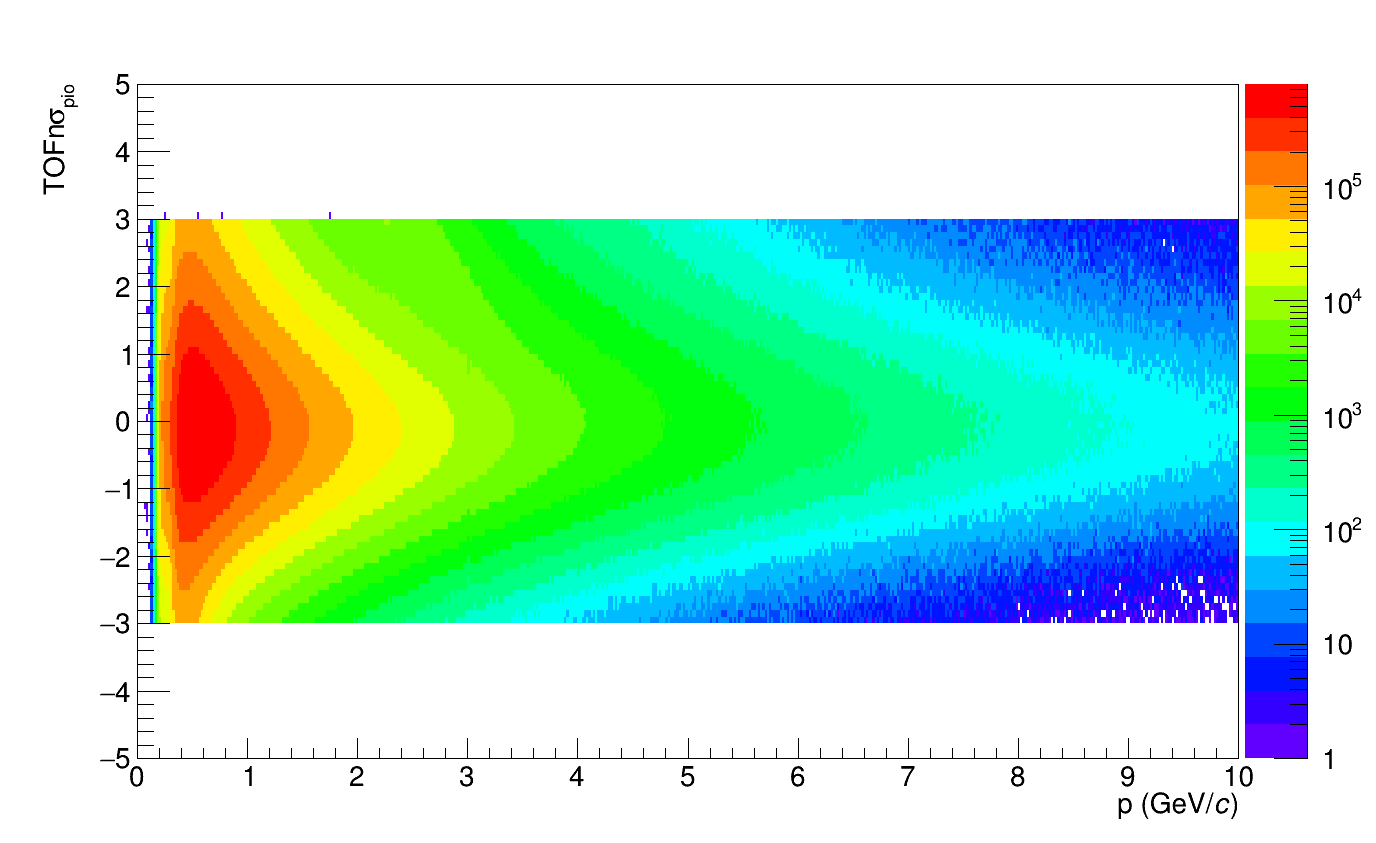
\includegraphics[width=0.98\linewidth]{Figures/ChargedPioCuts/TOFnsigmapioneg.png}
\caption{$n\sigma_{\pi}$ versus $p$ plot for the assumption of a pion in the TOF}
\label{fig:ChpioTOF}
\end{subfigure}
\caption{The specific energy loss of the particles in the TPC and TOF expressed in terms of the $n\sigma$ discrimination variable plotted against the particle momentum, here only shown for the negative particles; the colour scale shows the number of counts}
\label{fig:PIDChPio}
\end{figure}


\subsection{MC Production}

\section{Results}
\label{sec:Results}


show $\rho$ peak which is by-product in charged pi-pi spectrum from 3pi $a_1$ channel. Try to properly fit with fitting script. might be difficult because of weird background, has already been measured in ALICE, e.g. \cite{ALICErho}.
\section{Outlook}
\label{sec:Outlook}


\bibliographystyle{unsrt}  
\bibliography{references}
%

\end{document}
